% Diese Datei muss mit Lualatex kompiliert werden.

\documentclass[
	paper=a4,
	fontsize=10pt,
	pagesize=auto,
	DIV=14,
	BCOR=20mm,
	headsepline,
	parskip=half
]{scrbook}


\newcommand{\mytitle}{Grundlagen der Elektrizität – Praxisheft}
\newcommand{\myauthor}{T. Jenni}
\newcommand{\mydate}{\today}
\newcommand{\mysubject}{Einführung in die Elektrizitätslehre für Schülerinnen und Schüler}
\newcommand{\mykeywords}{Elektrizität, Physik, Praxisheft, Schaltungen, Ohmsches Gesetz}


% FONTS UND SPRACHE
\usepackage{fontspec}
\usepackage{polyglossia}
\setdefaultlanguage[spelling=new,babelshorthands=true]{german}

% MATHEMATIK UND NATURWISSENSCHAFT
\usepackage{mathtools}					% loads amsmath, e.g. pmatrix*
\usepackage{unicode-math}				% e.g. mathbb
\usepackage{siunitx}		            % SI-Unit package


% GRAFIK UND BILD
\usepackage{graphicx}					% bitmap graphics
\usepackage{tikz}						% vector graphics
\usetikzlibrary{calc}
\usepackage{pgfplots}					% plotting
\pgfplotsset{compat=1.18}
\usepgfplotslibrary{groupplots}


% LAYOUT UND DESIGN
\usepackage{scrlayer-scrpage}			% koma script package
\usepackage{tabularx}					% full width tables
\usepackage{makecell}					% controll tablecell size
\usepackage[most]{tcolorbox}	        % fancy boxes
\usepackage{subcaption}
\usepackage{pageslts}


% TEXTERWEITERUNGEN UND SONSTIGES
\usepackage[plainpages=false,pdfpagelabels]{hyperref}	% urls
\usepackage{bookmark} 					%
\usepackage{cancel}						% cancel chars
\usepackage{comment}					% comments
\usepackage[normalem]{ulem}		        % underline
\usepackage{environ}					% better environment
\usepackage{qrcode}						% generate qrcodes
\usepackage{xcolor}						% colors
\usepackage{emoji}						% insert emoji



%*********************
% INITIALISIERUNGEN
%*********************

% siunitx
\sisetup{
	output-decimal-marker = {.},
	per-mode = symbol,
	separate-uncertainty = false,
	add-decimal-zero = true,
	exponent-product = \cdot,
	round-mode=none
}

% hyperref
\hypersetup{pdfencoding=auto}
\hypersetup{
  pdftitle={\mytitle},
  pdfauthor={\myauthor},
  pdfsubject={\mysubject},
  pdfkeywords={\mykeywords}
}

% set * to \cdot in math mode
\mathcode`\*="8000
\begingroup
  \catcode`\*=\active
  \gdef*{\cdot}
\endgroup



%*******************
% LAYOUT
%*******************

% Nummerierung der Sections ohne Punkt (z. B. "1.1 Einleitung")
\renewcommand{\thesection}{\thechapter.\arabic{section}}
\renewcommand{\thesubsection}{\thesection.\arabic{subsection}}

% Keine Nummern in Kopfzeilen
\renewcommand*{\sectionmarkformat}{}

% Kopfzeilen-Schrift normal (nicht kursiv)
\setkomafont{pageheadfoot}{\normalfont}

% Abstand Kopf → Text
\headsep=1cm

% Scrlayer-Scrpage Kopf- und Fusszeilen aktivieren
\clearpairofpagestyles
\pagestyle{scrheadings}
\automark[section]{section}

% Kopfzeilen links/mitte/rechts (für gerade/ungerade Seiten identisch)
\ihead{\myauthor}
\chead{\headmark}
\ohead{\mydate}

% Fusszeile mit Seitenzahl z. B. 5 / 24
\pagenumbering{arabic}
\cfoot{\hfill \thepage\ / \lastpages{arabic}{1}}



%************************
%* LAYOUT KONFIGURATION *
%************************

% Nummerierungen
\renewcommand{\thefigure}{\arabic{figure}}
\renewcommand{\thetable}{\arabic{table}}
\renewcommand{\theequation}{\arabic{equation}}

% Beschriftungen (deutsch)
\addto\captionsgerman{%
  \renewcommand{\figurename}{Abb.}%
  \renewcommand{\tablename}{Tab.}%
}

% Kurzreferenzen
\newcommand{\fref}[1]{Abb.~\ref{#1}}
\newcommand{\tref}[1]{Tab.~\ref{#1}}

% Setze Emoji Schriftart
\setemojifont{TwemojiMozilla}



%**************************
% DEFINITIONEN UND MAKROS *
%**************************

\newtcolorbox{greenbox}{
    enhanced,
    boxrule=0pt,frame hidden,
    borderline west={4pt}{0pt}{green!75!black},
    colback=green!10!white,
    sharp corners
}

\newtcolorbox{redbox}{
    enhanced,
    boxrule=0pt,frame hidden,
    borderline west={4pt}{0pt}{red!75!black},
    colback=red!10!white,
    sharp corners
}



\newcounter{exercise}
\setcounter{exercise}{1}
\newcommand{\exercise}[2][pencil]{
    \subsection*{\makebox(0,0)[r]{\huge\emoji{#1}\hspace{1em}}Aufgabe \theexercise\  -- #2}
    \addtocounter{exercise}{1}
}

\newcounter{experiment}
\setcounter{experiment}{1}
\newcommand{\experiment}[2][screwdriver]{
    \subsection*{\makebox(0,0)[r]{\rotatebox[origin=c]{270}{\huge\emoji{#1}}\hspace{1em}}Experiment \theexperiment\  -- #2}
    \addtocounter{experiment}{1}
}


\newcommand{\marker}{\fontspec{Marker Felt}\fontsize{5mm}{8mm}\selectfont}

\newcommand{\markertable}{\fontspec{Marker Felt}\fontsize{5mm}{12mm}\selectfont}


\newif\ifshowanswers
\showanswerstrue % oder \showanswersfalse

\newcommand{\answer}[1]{\ifshowanswers #1 \fi}
\newcommand{\noanswer}[1]{\ifshowanswers \else #1 \fi}



\showanswersfalse % \showanswerstrue oder \showanswersfalse

\begin{document}


\begin{titlepage}
    \centering

    \vspace*{2.5cm}

    {\Huge\bfseries Grundlagen der Elektrizität \par}
    \vspace{0.5cm}
    {\Large\scshape Praxisheft für den Physikunterricht \par}

    \vspace{1.5cm}
    \includegraphics[width=9cm]{_images/visual}

    {Foto: Alex Suprun / Unsplash \par}

    \vfill

    {\large\itshape T. Jenni\\
    Kantonsschule Zug \par}

    \vspace{1cm}
    {\large \mydate \par}


\end{titlepage}

\renewcommand{\contentsname}{Inhalt}
\tableofcontents

\chapter{Einleitung}

Elektrizität ist in unserem Alltag allgegenwärtig. Sie findet Anwendung in Handys,
Computer, Haushaltsgeräte, Autos, Züge und Flugzeuge, um einige Beispiele zu nennen.
Elektrizität ist eine der wichtigsten Energieformen, die wir nutzen.

Neben der technischen Anwendung hat die Elektrizitätslehre auch eine grosse
Bedeutung in der Physik und ist zentral für das grundlegende Naturverständnis.
Die elektromagnetische Kraft ist eine der vier Grundkräfte der Physik.
Das Atom besteht aus einem elektrisch positiv geladenen Atomkern und
elektrisch negativ geladenen Elektronen, die den Atomkern umkreisen.

Dieses Dossier gibt dir eine Einführung in die Elektrizitätslehre.
Dabei wird nicht nur das theoretische Wissen vermittelt, sondern auch
praktische Experimente durchgeführt. Das Dossier enthält die folgenden
Abschnitte:

Im ersten Teil werden die Komponenten eines Stromkreises vorgestellt.
Der Unterschied zwischen Serie- und Parallelschaltung wird erklärt. Im zweiten
Teil werden die Grössen Stromstärke und Spannung eingeführt und erklärt,
wie sie gemessen werden können. Im dritten Teil wird auf die elektrische
Leistung und den elektrischen Widerstand eingegangen. In diesem Zusammenhang
wird das Ohm'sche Gesetz vorgestellt.


\vspace{1cm}

\begin{redbox}
Es ist wichtig, nur die vorgesehenen Bauteile zu verwenden und
nur die gezeigten Schaltungen aufzubauen. Bei unsachgemässer Verwendung
kann es zu Kurzschlüssen und Beschädigungen kommen.
\end{redbox}



\newpage
\section{Bauteile des Experimentierkastens}

Der Experimentierkasten enthält verschiedene Bauteile, siehe
\fref{fig:components}. Es gibt zwei Batteriehalter, zwei Schalter und
zwei Lampenhalter. Weiter sind zwei Messgeräte, ein Amperemeter und ein Voltmeter vorhanden.
Es gibt vier feste Widerstände und einen variablen Widerstand. Verbunden werden kann
alles mit Kabeln.



\begin{figure}[h!]
    \centering
    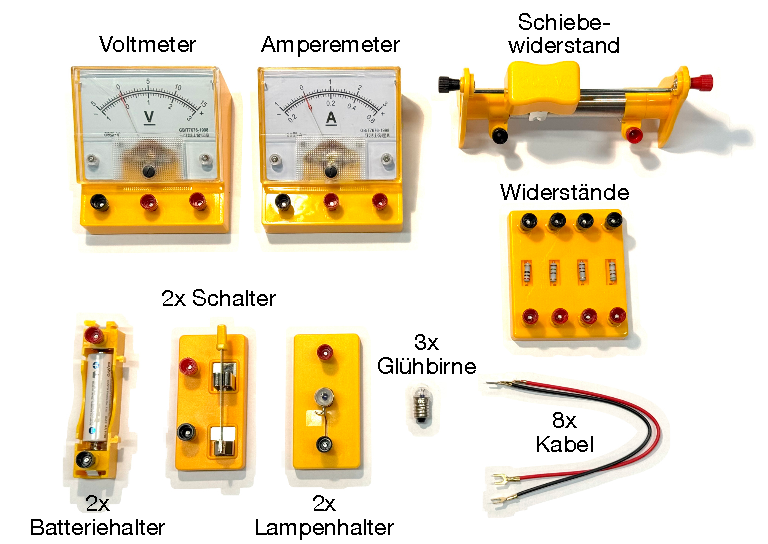
\includegraphics[width=12cm]{_images/bauteile.pdf}
    \caption{Bauteilübersicht}
    \label{fig:components}
\end{figure}


\section{Kabel anschliessen}

Die einzelnen Bauteile des Stromkreises können mit den Kabeln verbunden werden.
Dazu muss die Schraube im Gegenuhrzeigersinn gedreht werden. Anschliessend kann
das Kabel mit dem U-förmigen Anschluss verbunden werden. Die Schraube wird
wieder im Uhrzeigersinn gedreht, um das Kabel zu fixieren, siehe \fref{fig:connecting_wires}.

\begin{figure}[h!]
    \centering
    \begin{tikzpicture}
        \node[anchor=north west] at (0,0) {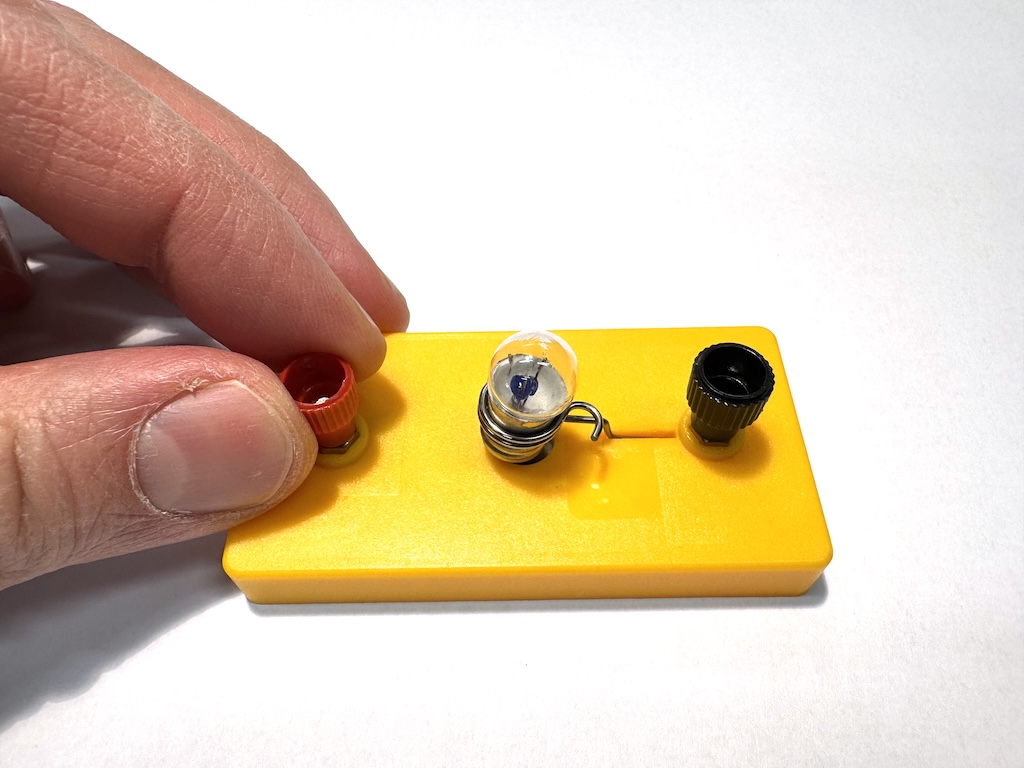
\includegraphics[width=4cm]{_images/kabel_anschliessen_1}};

        \node[anchor=north west] at (6,0) {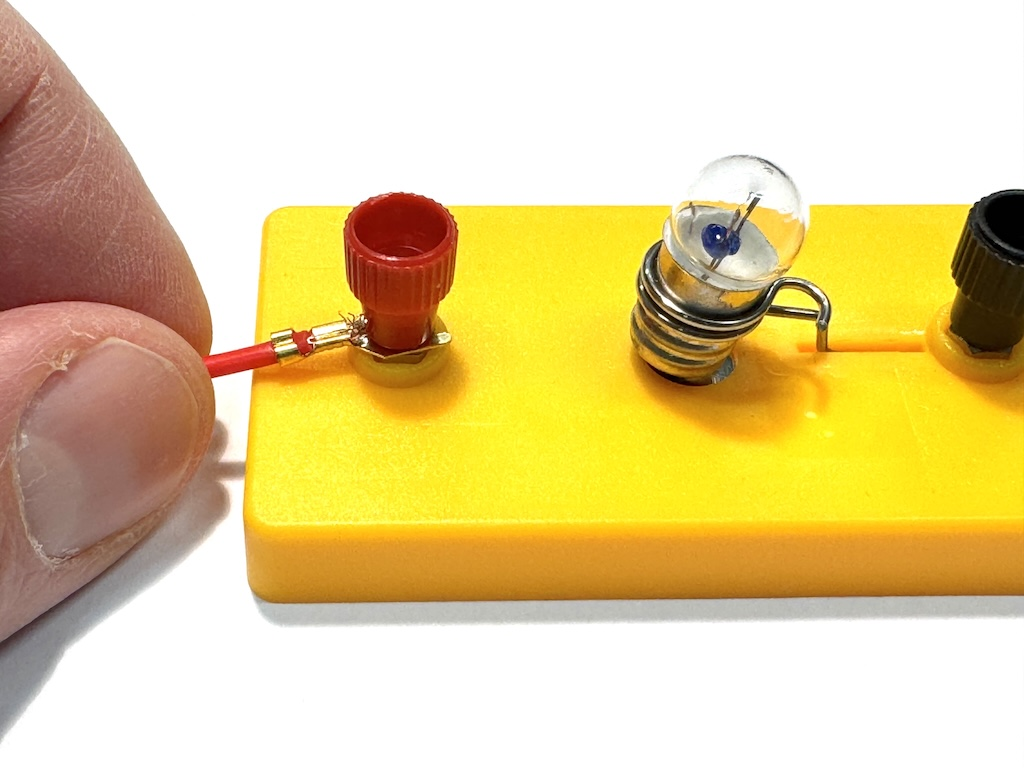
\includegraphics[width=4cm]{_images/kabel_anschliessen_2}};

        \node[anchor=north west] at (11,0) {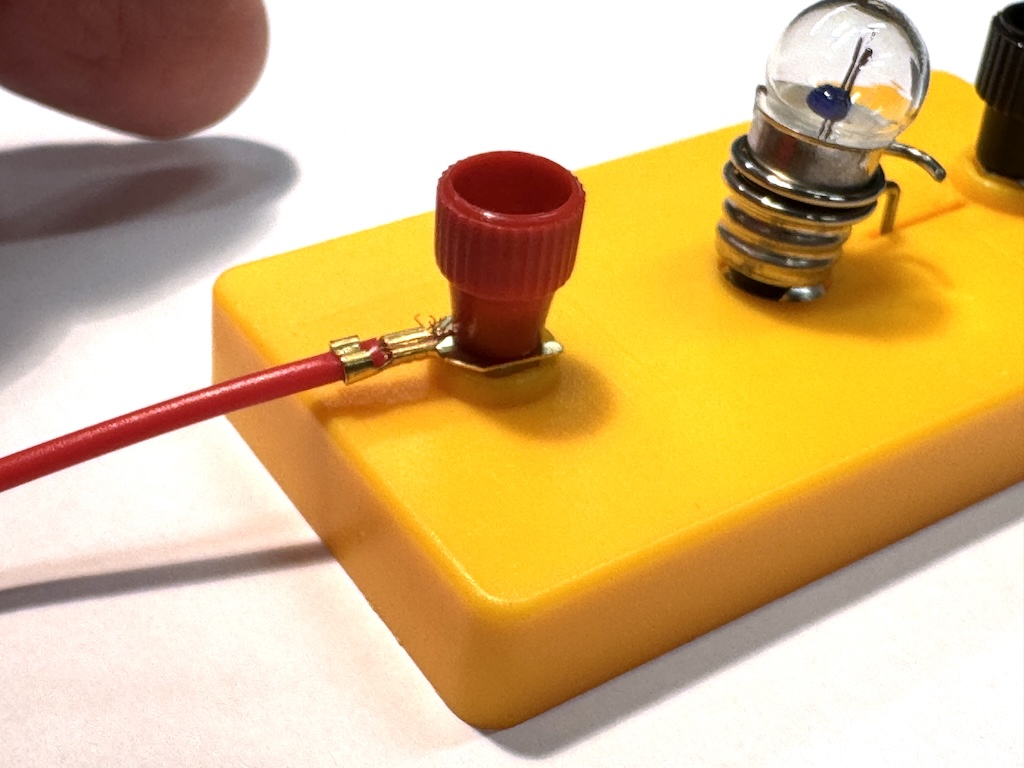
\includegraphics[width=4cm]{_images/kabel_anschliessen_3}};

        \node[anchor=south west] at (0,0) {1.};

        \node[anchor=south west] at (6,0) {2.};

        \node[anchor=south west] at (11,0) {3.};

    \end{tikzpicture}

    \caption{Kabel anschliessen}
    \label{fig:connecting_wires}
\end{figure}


\newpage
\section{Batterie}

Die Batterie muss korrekt in die Halterung eingesetzt werden.
Der Pluspol der Batterie muss bei dem roten Anschluss und der Minuspol
bei dem schwarzen Anschluss zu liegen kommen, siehe \fref{fig:batteryholder}.
Die Feder im Batteriehalter muss immer den Minuspol der Batterie berühren.

\begin{figure}[h!]
    \centering
    \begin{tikzpicture}
        \node[anchor=north west] at (0,0) {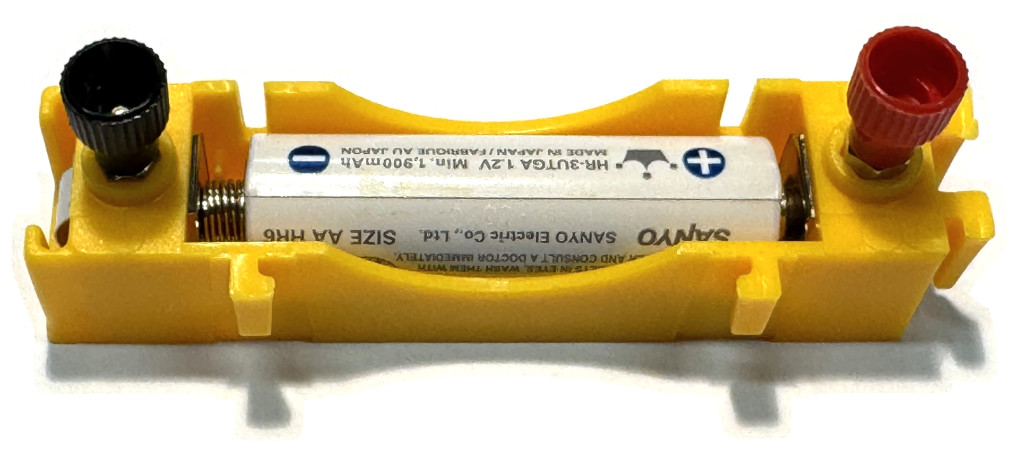
\includegraphics[width=6cm]{_images/batterie_solo}};

        \node[anchor=east] at (0.25,-0.75) {Minuspol (--)};

        \node[anchor=west] at (6.25,-0.75) {(+) Pluspol};

    \end{tikzpicture}

    \caption{Batteriehalter}
    \label{fig:batteryholder}
\end{figure}

Die Batteriehalter sind so konstruiert, dass sie in Serie oder parallel
zusammen geschaltet werden können, siehe \fref{fig:batteryholder_serial} und \fref{fig:batteryholder_parallel}.

\begin{figure}[h!]
    \centering
    \begin{subfigure}[b]{0.4\textwidth}
    \centering
    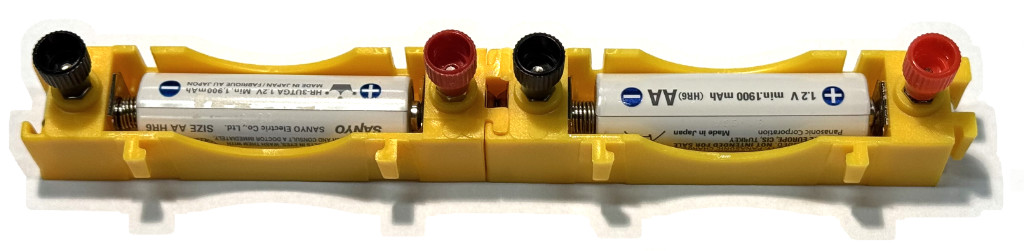
\includegraphics[width=7cm]{_images/batterie_seriell}
    \caption{\label{fig:batteryholder_serial}}
    \end{subfigure}
    \quad
    \begin{subfigure}[b]{0.4\textwidth}
    \centering
    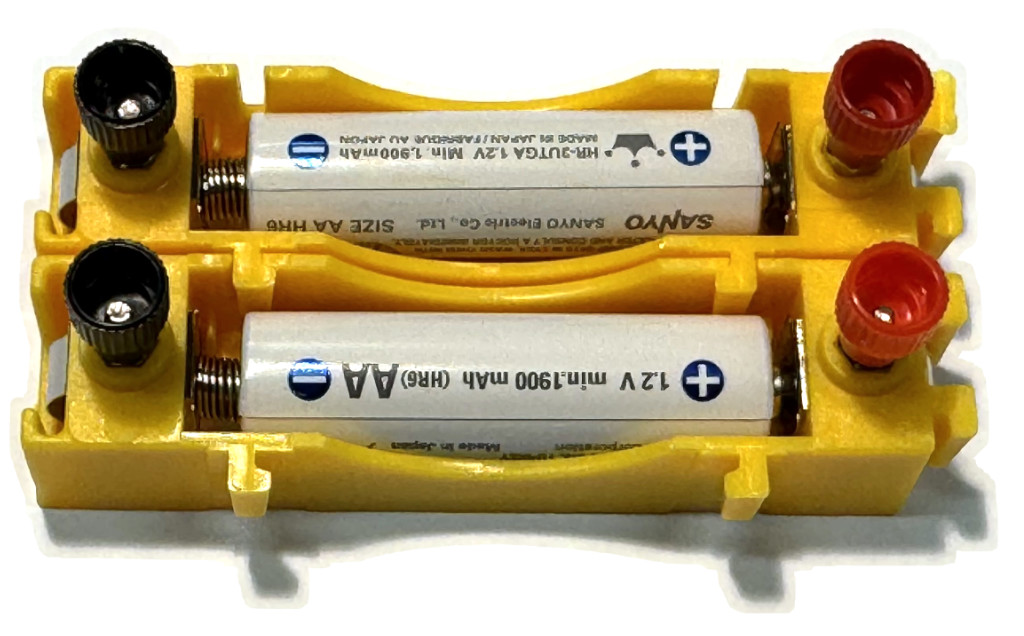
\includegraphics[width=3.8cm]{_images/batterie_parallel}
    \caption{\label{fig:batteryholder_parallel}}
    \end{subfigure}

    \caption{Serienschaltung (a) und Parallelschaltung (b) von Batterien}
\end{figure}


\section{Schaltsymbole}

In der Elektrizität werden Schaltsymbole verwendet, um die Teile des
Stromkreises darzustellen. Hier ist eine Übersicht über einige Schaltsymbole,
welche in diesem Dossier vorkommen.

\begin{figure}[h!]
    \centering
    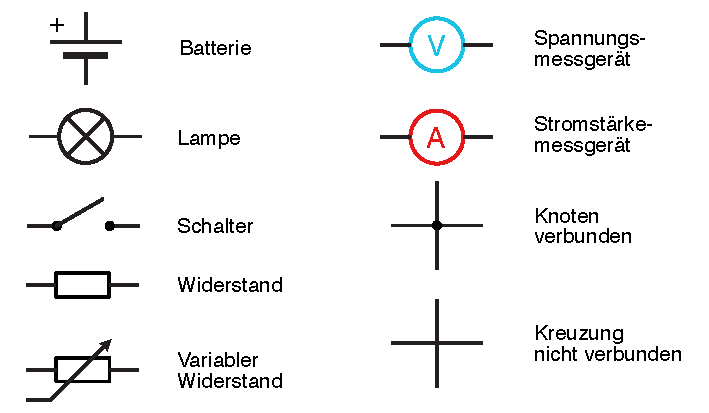
\includegraphics[width=10cm]{_images/schaltsymbole.pdf}
    \caption{Übersicht über alle Schaltsymbole}
    \label{fig:symbols}
\end{figure}


\newpage
\chapter{Stromkreis}

In der \fref{fig:circuit_battery} ist ein Stromkreis gezeigt.
Er besteht aus einer Spannungsquelle (Batterie), einem Verbraucher (Glühlampe)
und einem Hin- und einem Rückleiter (rotes und schwarzes Kabel).

Man kann einen Stromkreis auch als Schaltplan darstellen, siehe \fref{fig:circuit_schematic}.
Die Spannungsquelle ist durch ein Batteriesymbol und der Verbraucher durch ein
Lämpchensymbol dargestellt Verbunden sind sie durch die Kabel, welche
als durchgezogene Linien dargestellt werden.

\begin{figure}[h!]
\centering
    \begin{subfigure}[b]{0.46\textwidth}
    \centering
    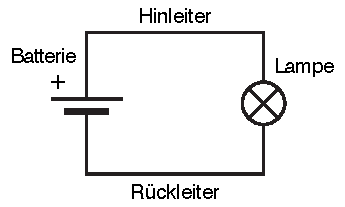
\includegraphics[width=6cm]{_images/stromkreis_schaltplan}
    \caption{\label{fig:circuit_schematic}}
    \end{subfigure}
\quad
    \begin{subfigure}[b]{0.46\textwidth}
    \centering
    \includegraphics[width=5.5cm]{_images/stromkreis_batterie}
    \caption{\label{fig:circuit_battery}}
    \end{subfigure}

    \caption{Schaltplan und Aufbau eines Stromkreises}
\end{figure}

Eine Spannungsquelle (Batterie) erzeugt eine elektrische Spannung, die
die Elektronen in den Kabel in Bewegung setzen. Die Elektronen bewegen sich durch die
Kabel und durch die Verbraucher (Glühlampe). Die Verbraucher sind Geräte, die
elektrische Energie in andere Energieformen umwandeln, z.B. in Wärme,
Licht oder Bewegung.





\newpage
\experiment{Einfacher Stromkreis}

Baue das Experiment aus siehe \fref{fig:experiment_circuit} auf. Verwende eine Batterie, eine Glühbirne und einen Schalter.
Beachte, dass die Batterie so eingebaut wird, dass der Pluspol beim roten und der Minuspol
beim schwarzen Anschluss zu liegen kommt. Schliesse den Stromkreis und beobachte, was passiert.

\begin{figure}[h!]
    \centering
    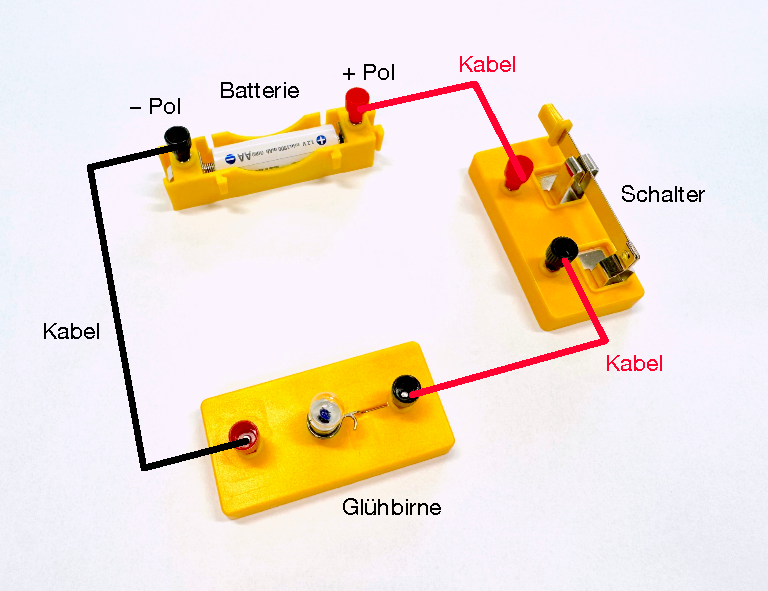
\includegraphics[width=9cm]{_images/stromkreis.pdf}
    \caption{Stromkreis}
    \label{fig:experiment_circuit}
\end{figure}

Beantworte die folgende Fragen: Was passiert, wenn ...

\begin{enumerate}
    \item ein Kabel aus dem Stromkreis entfernt wird?
    \item die Batterie umgedreht wird?
    \item der Schalter und die Glühbirne vertauscht werden?
\end{enumerate}

% Raster für die Antworten
\begin{tikzpicture}
    \draw[step=4mm,gray,very thin] (0,0) grid (14.8,-7.6);

    \answer{
        \draw (0.3,0.14) node[anchor=north west,align=left,text width=13cm] {%
    		\marker%

            \textbf{1.} Wenn ein Kabel entfernt wird, erlischt das Lämpchen.\\
            \textbf{2.} Wenn die Batterie umgedreht wird, ändert sich nichts.\\
            \textbf{3.} Wenn Schalter und Glühbirne vertauscht werden, ändert sich nichts.\\
        };
    }
\end{tikzpicture}


\newpage
\section{Das Wassermodell eines Stromkreises}
Es gibt eine Analogie zwischen einem Stromkreis und einem Wasserkreislauf.
Das Wasser wird mit einem Schöpflöffel (Batterie) von dem Behälter
mit tieferem Wasserstand (Minuspol) in den Behälter mit höherem Wasserstand
(Pluspol) geschöpft. Durch das Gefälle fliesst das Wasser durch die Rohre
(Kabel) und treibt das Wasserrad (Glühlampe) an, siehe \fref{fig:watermodel}.
Der Schalter entspricht einem Ventil, das den Wasserfluss unterbricht.


\begin{figure}[h!]
    \centering
    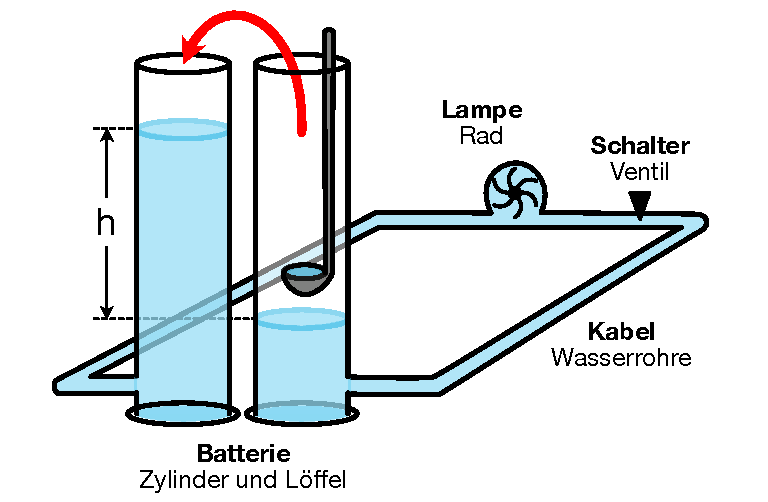
\includegraphics[width=11cm]{_images/wassermodell_stromkreis.pdf}
    \caption{Analogie: Wassermodell eines Stromkreises}
    \label{fig:watermodel}
\end{figure}

Lässt man das Wasser fliessen, ohne Wasser nachzuschöpfen, gleichen sich
die Wasserstände in den Behältern langsam an und das Wasserrad dreht langsamer.
Nach einer gewissen Zeit werden sich die Wasserstände in den Behältern gleich
sein und es fliesst kein Wasser mehr. Die Batterie ist nun leer und muss wieder
mit dem Schöpflöffel aufgefüllt werden.






\newpage
\exercise{Die Wirkungen vom elektrischen Strom}

Strom kann unter anderem Licht, Wärme, Schall, Bewegung und Magnetismus erzeugen.
Verbinde die Wirkungen mit den Geräten, die sie erzeugen.

\begin{tikzpicture}
    \draw[step=4mm,lightgray,very thin] (0,0) grid (14.8,-20);



    \node[fill=white,draw,very thick,inner sep=0.5cm,rounded corners, rotate=-2] (motion) at (3,-2) {\marker%
        Bewegung
    };

    \node[fill=white,draw,very thick,inner sep=0.5cm,rounded corners, rotate=2] (sound) at (3,-6) {\marker%
        Schall
    };

    \node[fill=white,draw,very thick,inner sep=0.5cm,rounded corners, rotate=3] (heat) at (3,-10) {\marker%
        Wärme
    };

    \node[fill=white,draw,very thick,inner sep=0.5cm,rounded corners, rotate=2] (magnet) at (3,-14) {\marker%
        Magnetismus
    };

    \node[fill=white,draw,very thick,inner sep=0.5cm,rounded corners, rotate=-1] (light) at (3,-18) {\marker%
        Licht
    };


    \node[rotate=3] (speaker) at (11,-2)
        {
\includegraphics[width=5cm]{_images/wirkung_lautsprecher}}; % Eric Nopanen / Unsplash

    \node[rotate=1] (lamp) at (12,-6)
            {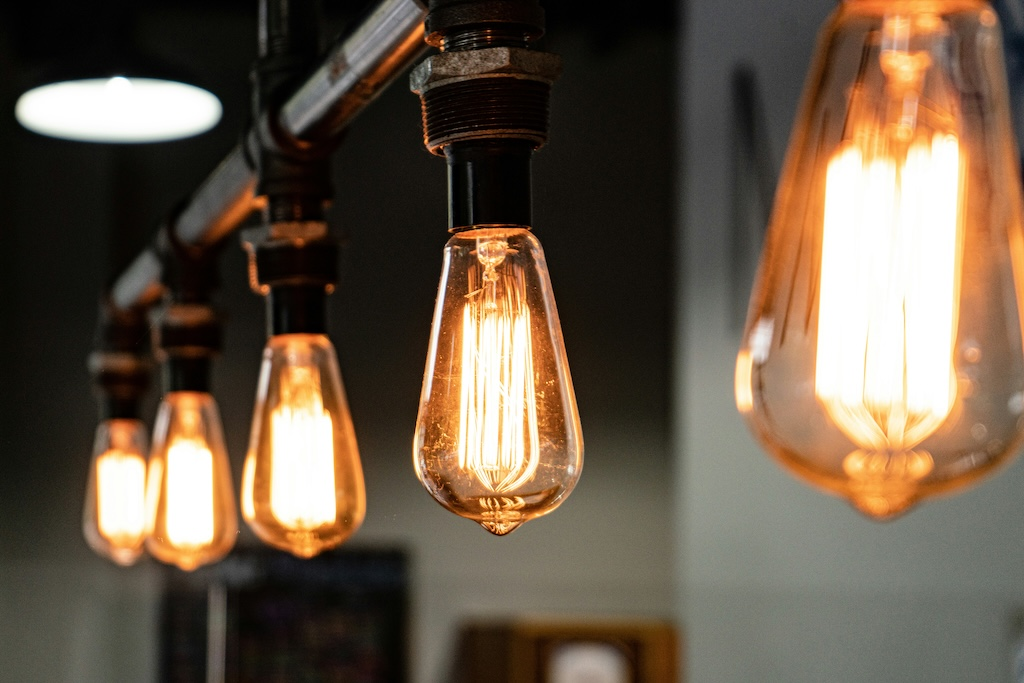
\includegraphics[width=5cm]{_images/wirkung_lampe}}; % Daniel Herron / Unsplash

    \node[rotate=-2] (fan) at (11,-10)
            {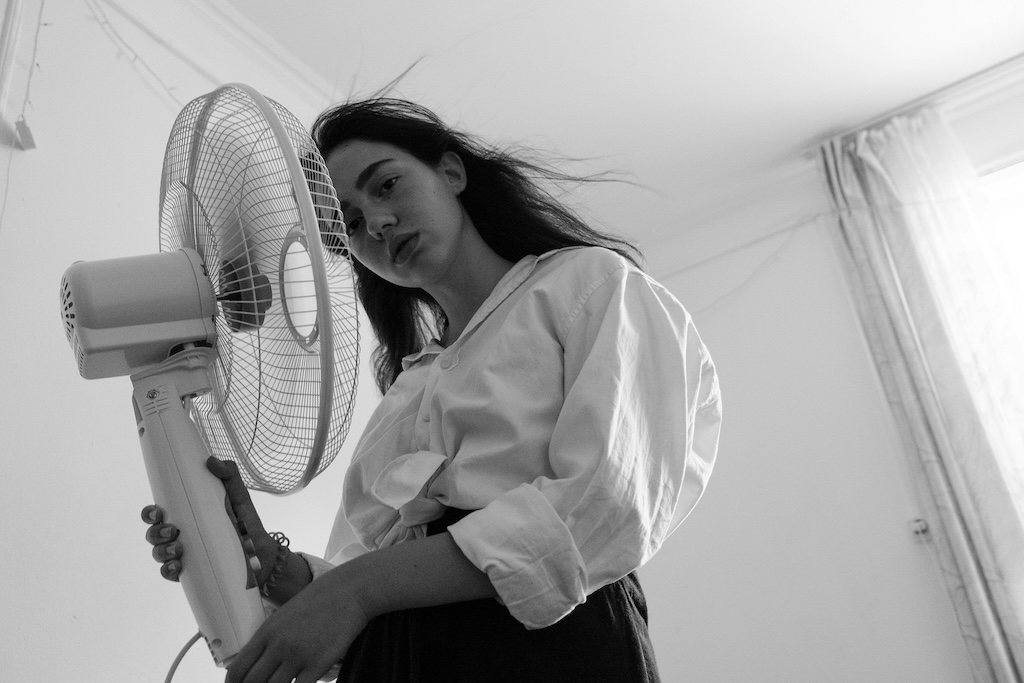
\includegraphics[width=5cm]{_images/wirkung_ventilator}}; % Daniil Onischenko / Unsplash

    \node[rotate=-3] (toaster) at (12,-14)
            {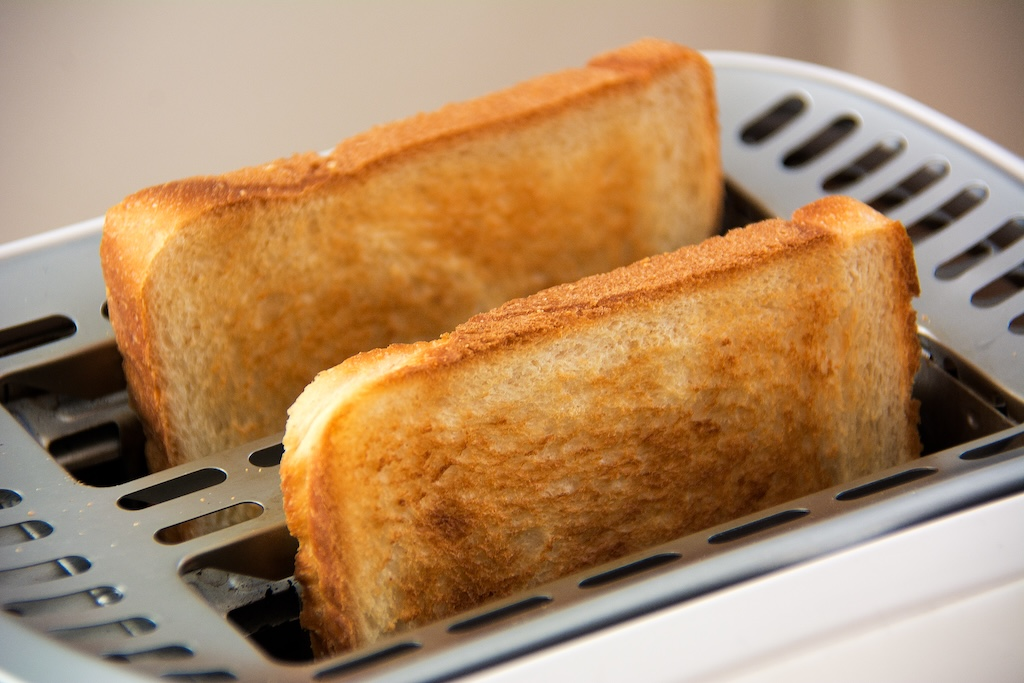
\includegraphics[width=5cm]{_images/wirkung_toaster}}; % CC0 / pxhere.com

    \node[rotate=2] (crane) at (11,-18)
            {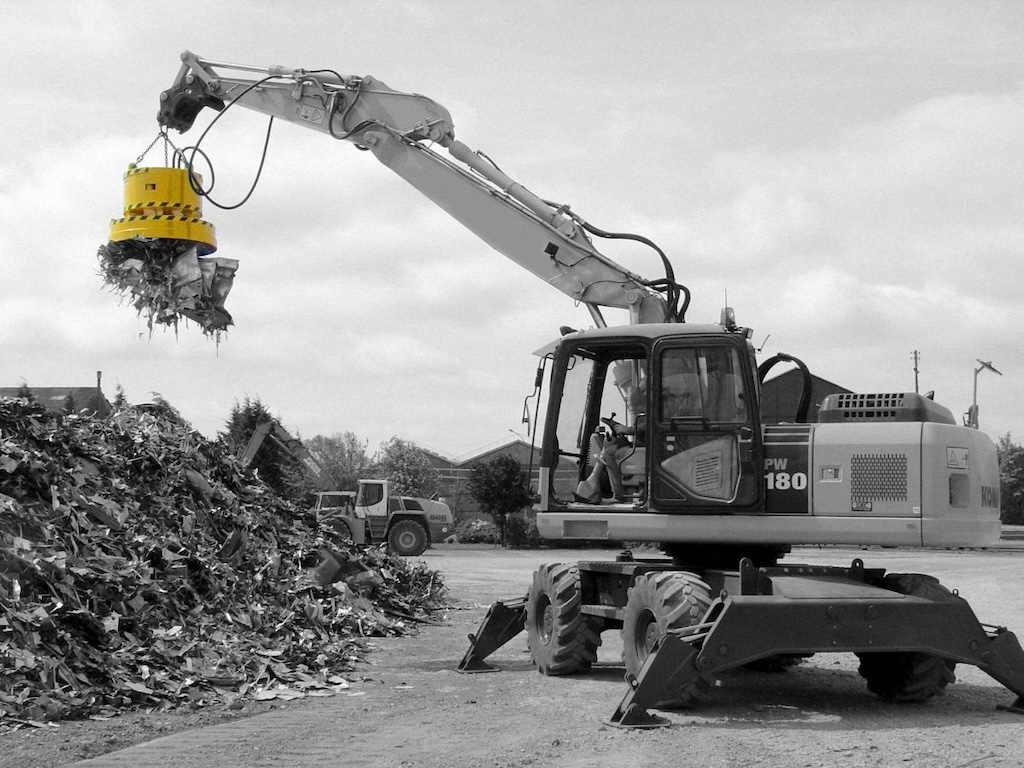
\includegraphics[width=5cm]{_images/wirkung_magnet}}; % hvrmagnet.com


    \answer{
        \draw [very thick, dashed]
            (heat.east) .. controls ++(0:2) and ++(180: 2) .. (speaker.west)
            (heat.east) .. controls ++(0:2) and ++(180: 2) .. (lamp.west)
            (heat.east) .. controls ++(0:2) and ++(180: 2) .. (fan.west)
            (heat.east) .. controls ++(0:2) and ++(180: 2) .. (crane.west);

        \draw [very thick]
            (motion.east) .. controls ++(0:2) and ++(180: 2) .. (fan.west)
            (sound.east) .. controls ++(0:2) and ++(180: 2) .. (speaker.west)
            (heat.east) .. controls ++(0:2) and ++(180: 2) .. (toaster.west)
            (light.east) .. controls ++(0:2) and ++(180: 2) .. (lamp.west)
            (magnet.east) .. controls ++(0:2) and ++(180: 2) .. (crane.west);

    }


\end{tikzpicture}



\newpage
\section{Serien- und Parallelschaltung}

Bei der <<Serienschaltung>> oder <<Reihenschaltung>> sind die Verbraucher
wie in einer Kette hintereinander angeordnet. Der gleiche elektrische Strom fliesst
durch alle Verbraucher nacheinander. Es gibt keine Verzweigungen und somit
nur einen Stromkreis. Ein Beispiel für ist eine Lichterkette
der Weihnachtsbeleuchtung, siehe \fref{fig:christmaslights}.

\begin{figure}[h!]
\centering
    \begin{subfigure}[b]{0.46\textwidth}
    \centering
    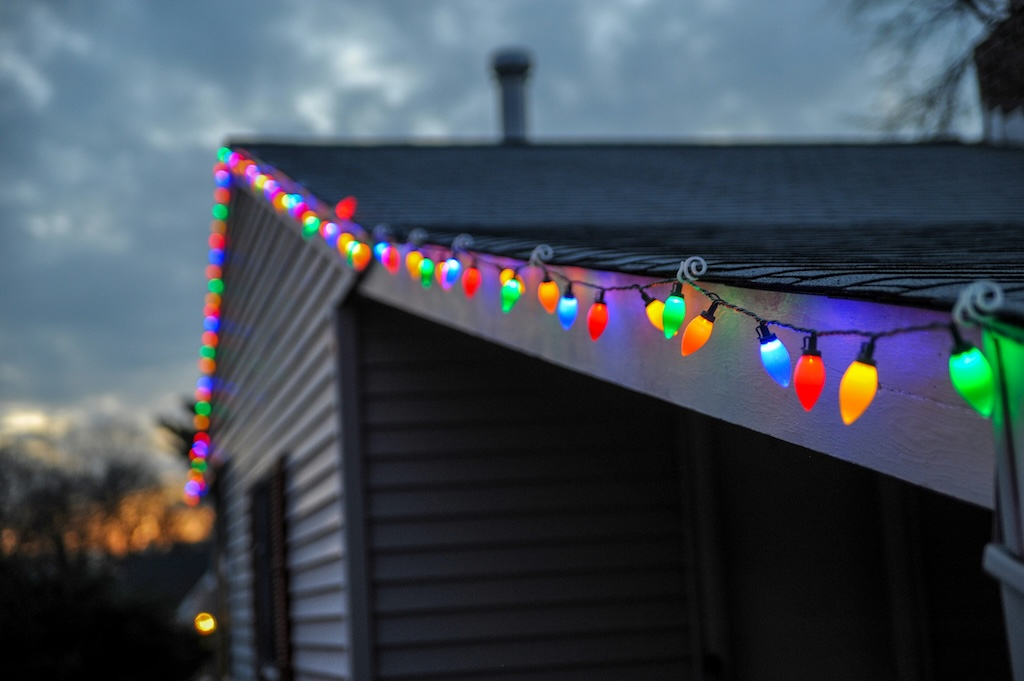
\includegraphics[width=6cm]{_images/weihnachtsbeleuchtung}
    \caption{\label{fig:christmaslights}}
    \end{subfigure}
    \quad
    \begin{subfigure}[b]{0.46\textwidth}
    \centering
    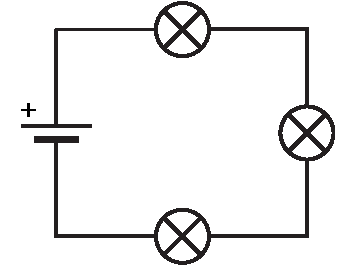
\includegraphics[width=5.5cm]{_images/serienschaltung_schaltplan}
    \caption{\label{fig:series_schematic}}
    \end{subfigure}

    \caption{Weihnachtsbeleuchtung und Schaltplan}
\end{figure}



Bei der <<Parallelschaltung>> sind die Verbraucher alle direkt an
die Spannungsquelle angeschlossen, siehe \fref{fig:parallel_schematic}.
Es gibt mehrere Knotenpunkte, an bei denen der Strom sich verzweigt.
Somit hat jeder Verbraucher seinen eigenen Stromkreis.
Ein Beispiel ist eine Steckdose, bei der mehrere Geräte angeschlossen werden
können, wie in \fref{fig:powerstrip} gezeigt.

\begin{figure}[h!]
\centering
    \begin{subfigure}[b]{0.46\textwidth}
    \centering
    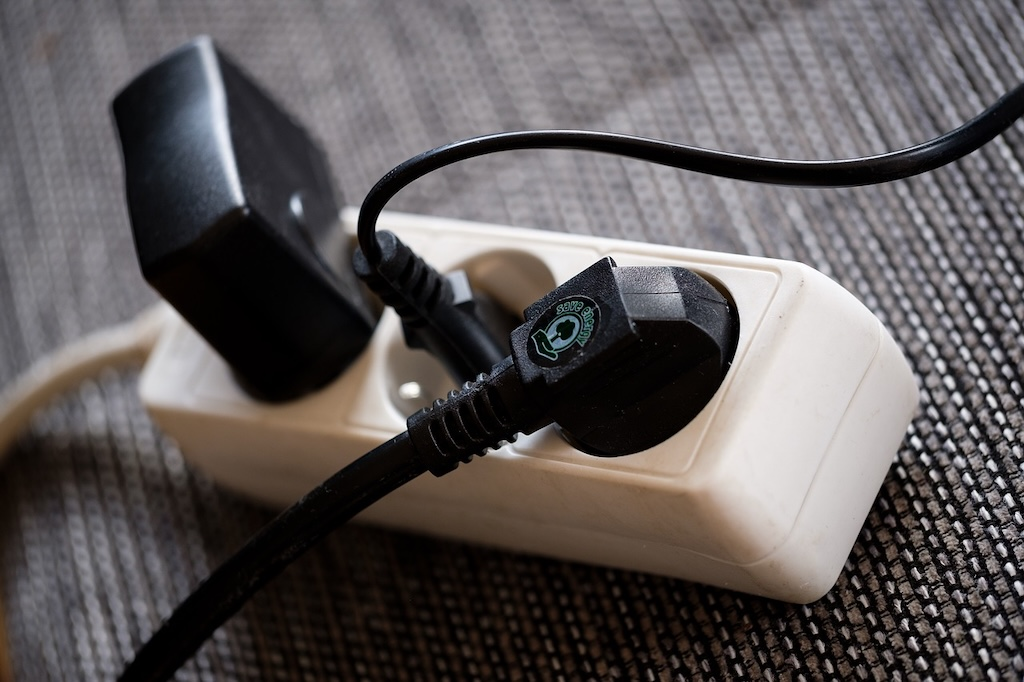
\includegraphics[width=6cm]{_images/steckdosenleiste}
    \caption{\label{fig:powerstrip}}
    \end{subfigure}
\quad
    \begin{subfigure}[b]{0.46\textwidth}
    \centering
    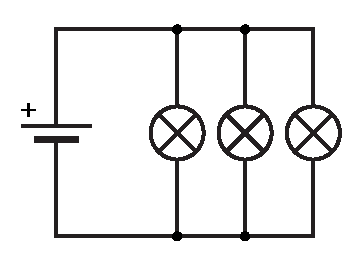
\includegraphics[width=5.5cm]{_images/parallelschaltung_schaltplan}
    \caption{\label{fig:parallel_schematic}}
    \end{subfigure}

    \caption{Weihnachtsbeleuchtung und Steckdosenleiste}
\end{figure}



\newpage
\experiment{Serienschaltung}

Baue das Experiment aus siehe \fref{fig:experiment_lamps_series} auf. Die
Lampen und die Batteriensind nacheinander, d.h. in Serie geschaltet.

\begin{figure}[h!]
    \centering
    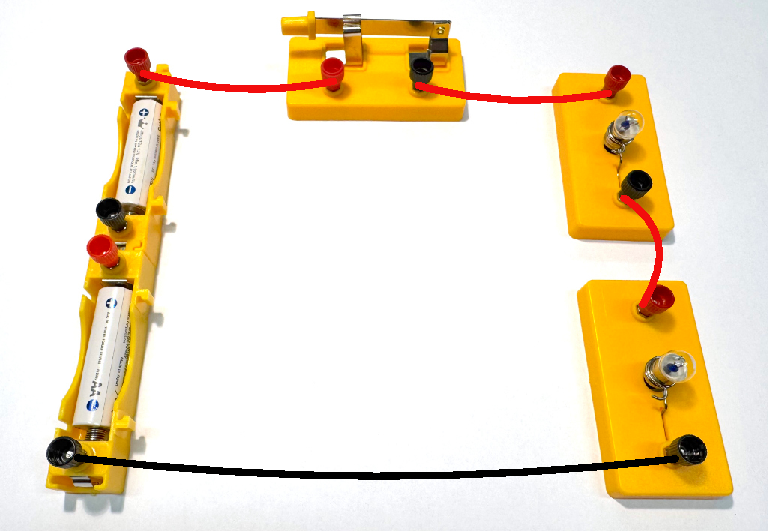
\includegraphics[width=9cm]{_images/lampen_serie.pdf}
    \caption{Lampen in einer Serienschaltung}
    \label{fig:experiment_lamps_series}
\end{figure}

Beantworte die folgenden Fragen:

\begin{enumerate}
    \item Was passiert, wenn ein Lämpchen <<kaputt>> geht. Drehe es dazu aus der Fassung.
    \item Was passiert, wenn du nur eine anstatt zwei Batterien verwendest?
    \item Vervollständige den Schaltplan.
\end{enumerate}

% Raster für die Antworten
\begin{tikzpicture}
    \draw[step=4mm,gray,very thin] (0,0) grid (14.8,-8.4);

    \noanswer{
        \node  at (7,-6)
            {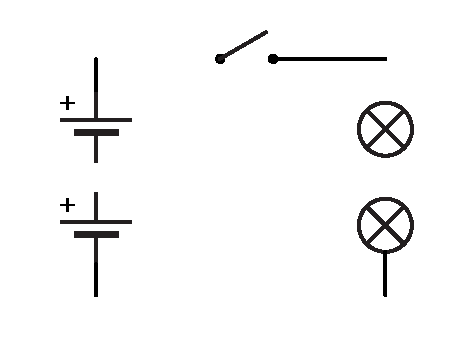
\includegraphics[width=8cm]{_images/lampen_serie_schaltplan.pdf}};
    }
    \answer{
        \node  at (7,-6)
            {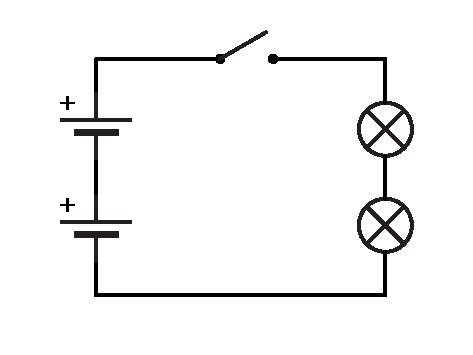
\includegraphics[width=8cm]{_images/lampen_serie_schaltplan_loesung.pdf}};
    }
    \answer{
        \draw (0.3,0.14) node[anchor=north west,align=left,text width=13cm] {%
            \marker%

            \textbf{1.} Wenn ein Lämpchen kaputt geht, erlischt das andere auch.\\
            \textbf{2.} Wenn man nur eine Batterie verwendet, brennen die Lämpchen nur noch ganz schwach. \\
        };
    }
\end{tikzpicture}





\newpage
\experiment{Parallelschaltung}

Baue das Experiment aus siehe \fref{fig:experiment_lamps_parallel} auf. Die
Lampen und die Batteriensind nebeneinander, d.h. in Parallel geschaltet.

\begin{figure}[h!]
    \centering
    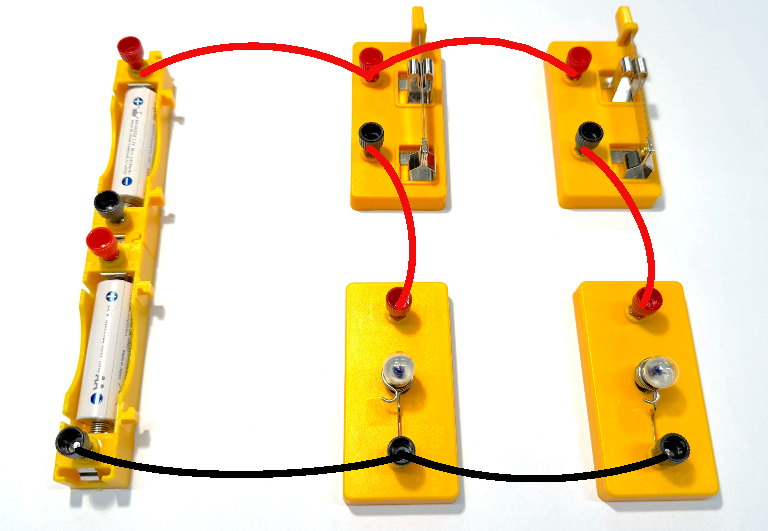
\includegraphics[width=9cm]{_images/lampen_parallel.pdf}
    \caption{Lampen in einer Parallelschaltung}
    \label{fig:experiment_lamps_parallel}
\end{figure}

Beantworte die folgenden Fragen:

\begin{enumerate}
    \item Wie hell leuchten die Lampen im Vergleich zu einer Serienschaltung?
    \item Was passiert, wenn ein Lämpchen kaputt geht. Drehe es dazu aus der Fassung.
    \item Vervollständige den Schaltplan.
\end{enumerate}

% Raster für die Antworten
\begin{tikzpicture}
    \draw[step=4mm,gray,very thin] (0,0) grid (14.8,-8.4);

    \noanswer{
        \node  at (7,-6)
            {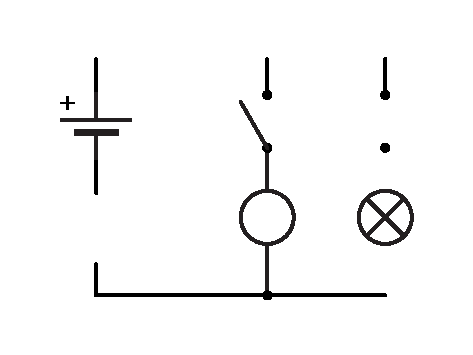
\includegraphics[width=8cm]{_images/lampen_parallel_schaltplan}};
    }
    \answer{
        \node  at (7,-6)
            {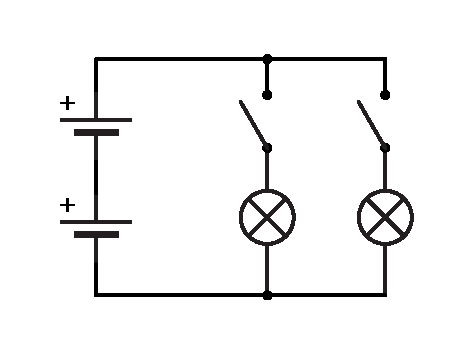
\includegraphics[width=8cm]{_images/lampen_parallel_schaltplan_loesung}};
    }
    \answer{
        \draw (0.3,0.14) node[anchor=north west,align=left,text width=13cm] {%
    		\marker%

            \textbf{1.} Die Lämpchen leuchten heller als in bei der Serienschaltung. \\
            \textbf{2.} Wenn ein Lämpchen kaputt geht, leuchtet das andere weiterhin.\\
        };
    }
\end{tikzpicture}


\exercise{In Serie oder Parallel?}

Bestimme bei den gezeigten Schaltplänen, ob die Lampen in Serie oder Parallel geschaltet sind.

\begin{tikzpicture}
    \draw[step=4mm,lightgray,very thin] (0,0) grid (14.8,-8);

    \node at (0.6,-0.5) {a)};
    \node at (3.5,-3)
            {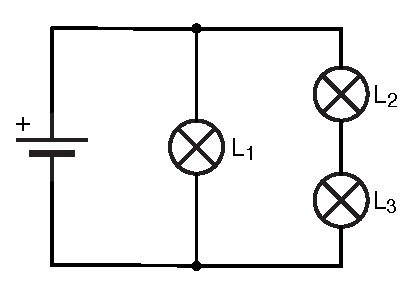
\includegraphics[width=7cm]{_images/serie_parallel_aufgabe_1}};

    \node at (8.6,-0.5) {b)};
    \node at (11.5,-3)
            {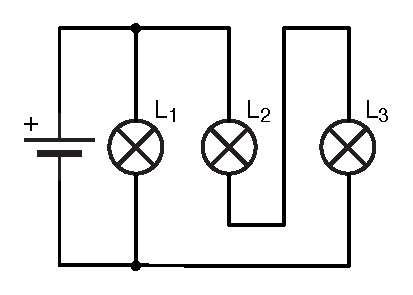
\includegraphics[width=7cm]{_images/serie_parallel_aufgabe_2}};


    \answer{
        \draw (0.3,-5.14) node[anchor=north west,align=left,text width=13cm] {%
    		\marker%

            \textbf{a)} L$_{\text{2}}$ und L$_{\text{3}}$ sind zueinander parallel. L$_{\text{1}}$ ist in Serie zu L$_{\text{2}}$ und L$_{\text{3}}$. \\

            \textbf{b)} Gleich wie Aufgabe a)\\
        };
    }


\end{tikzpicture}






\section{Kurzschluss}

Manchmal kann es zu einem Kurzschluss kommen, wenn man aus Versehen eine direkte Verbindung
zwischen den Batteriepolen macht. In diesem Fall kann
es zu einem Überstrom kommen, welcher die Kabel oder die Batterie zerstört.

Wenn etwa ein Haushaltsgerät kaputtgeht, kann es auch zu einem Kurzschluss kommen.
Oft sind es alte Steckerleisten, welche nicht mehr richtigen Kontakt haben. Sie können
sich aufheizen und schmelzen, siehe \fref{fig:short_circuit}.

\begin{figure}[h!]
    \centering
    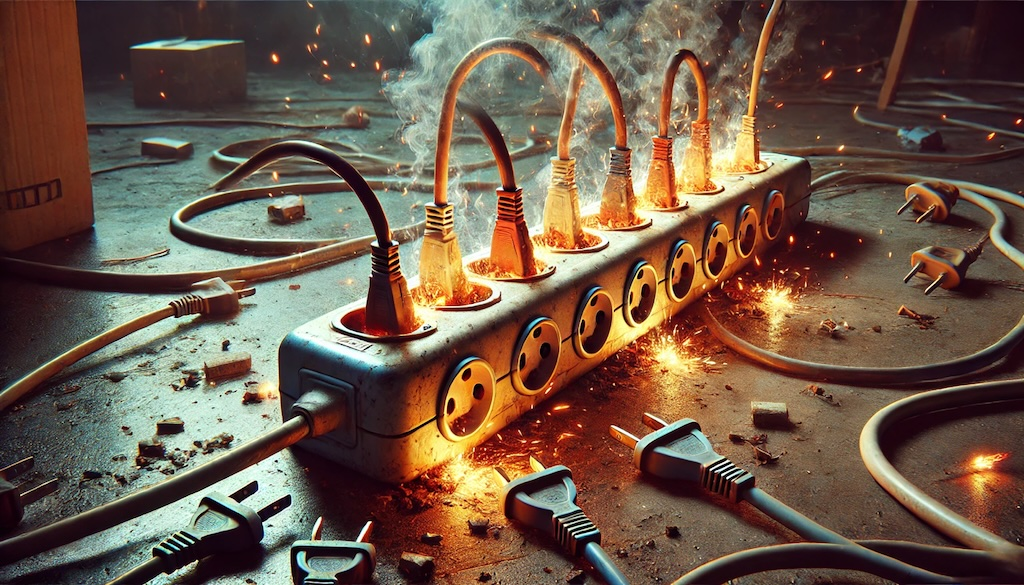
\includegraphics[width=9cm]{_images/kurzschluss}
    \caption{Kurzschluss bei einer Steckerleiste (Bild erstellt mit DALL·E, OpenAI)}
    \label{fig:short_circuit}
\end{figure}

\begin{redbox}
Kurzschlüsse müssen vermieden werden. Es ist wichtig, nur intakte Bauteile zu verwenden und
nur die gezeigten Schaltungen aufzubauen und vor dem Einschalten zu überprüfen.
\end{redbox}



\newpage
\experiment{Kurzschluss}


Baue das Experiment aus siehe \fref{fig:experiment_short_circuit} auf. Der Kurzschluss über
der rechten Lampe ist nicht gefährlich. Der gesamte Strom geht über das Kabel.
Eine Gefahr besteht, wenn man die Batteriepole direkt kurzschliesst.

\begin{figure}[h!]
    \centering
    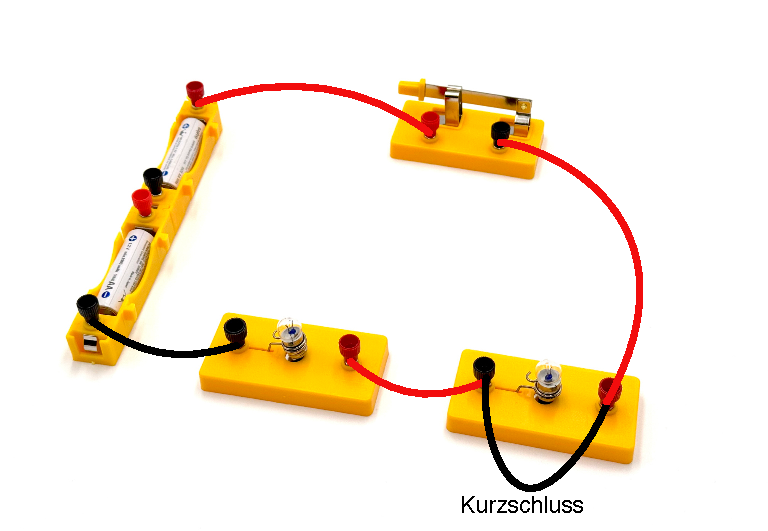
\includegraphics[width=9cm]{_images/kurzschluss_aufbau.pdf}
    \caption{Aufbau eines Kurzschlusses}
    \label{fig:experiment_short_circuit}
\end{figure}

Schliesse den Schalter und notiere deine Beobachtungen. Beantworte die folgenden Fragen:

\begin{enumerate}
    \item Was passiert mit der rechten Lampe?
    \item Was passiert, wenn du nur die linke Lampe kurzschliesst?
    \item Was bedeutet das für den elektrischen Strom?
\end{enumerate}

% Raster für die Antworten
\begin{tikzpicture}
    \draw[step=4mm,gray,very thin] (0,0) grid (14.8,-8.4);

    \answer{
        \draw (0.3,0.14) node[anchor=north west,align=left,text width=13cm] {%
    		\marker%

            1. Der Kurzschluss führt dazu, dass die rechte Lampe nicht leuchtet. Der gesamte Strom
            geht über das Kabel. \\
            \ \\
            2. Der Kurzschluss führt dazu, dass die linke Lampe nicht leuchtet. Der gesamte Strom
            geht über das Kabel. \\
            \ \\
            3. Der elektrische Strom nimmt immer den Weg mit der geringsten Widerstand. Man kann
            sagen, der elektrische Strom ist faul.
        };
    }
\end{tikzpicture}


\newpage
\chapter{Stromstärke- und Spannungsmessung}

Zwei der grundlegenden Grössen in der Elektriztitätslehre sind die Spannung $U$ und die Stromstärke $I$.
Ein elektrischer Strom entsteht, wenn sich elektrische Ladungen bewegen.
Die Spannung ist die Ursache dafür, dass diese sich bewegen. Ist die Spannung null, fliesst kein elektrischer Strom.

Im Wassermodell sieht
man das sehr gut, siehe \fref{fig:watermodel}. Ist der Höhenunterschied zwischen den Tanks null, fliesst kein
Wasser durch die Rohre.

Gibt es eine Spannung und ist der Stromkreis geschlossen, fliesst ein elektrischer Strom.
Die Stromstärke ist die Menge an Ladung, die durch einen bestimmten Zeitraum fliesst.
Im Wassermodell entspricht die Stromstärke der Flussrate des Wassers, d.h. wie viel Wasser pro Sekunde
an einer Stelle im Rohr durchfliesst.


\section{Stromstärkemessung}

Die Stromstärke $I$ ist definiert als das Verhältnis zwischen der Ladung $Q$ und der Zeit $t$,
die benötigt wird, um diese Ladung zu transportieren. Die Einheit der Stromstärke ist
Ampere ($\unit{\ampere}$).

\begin{greenbox}
\textbf{Stromstärke $I$}
$$
    I = \frac{Q}{t} \quad,\quad \left[ I \, \right] = \frac{\unit{\coulomb}}{\unit{\second}} = \unit{\ampere} \quad \text{(Ampere)}
$$
\end{greenbox}


Betrachten wir nun die Messung der elektrischen Stromstärke $I$. Man verwendet dazu ein
Stromstärkemessgerät, auch Amperemeter genannt.

\begin{figure}[h!]
    \centering
    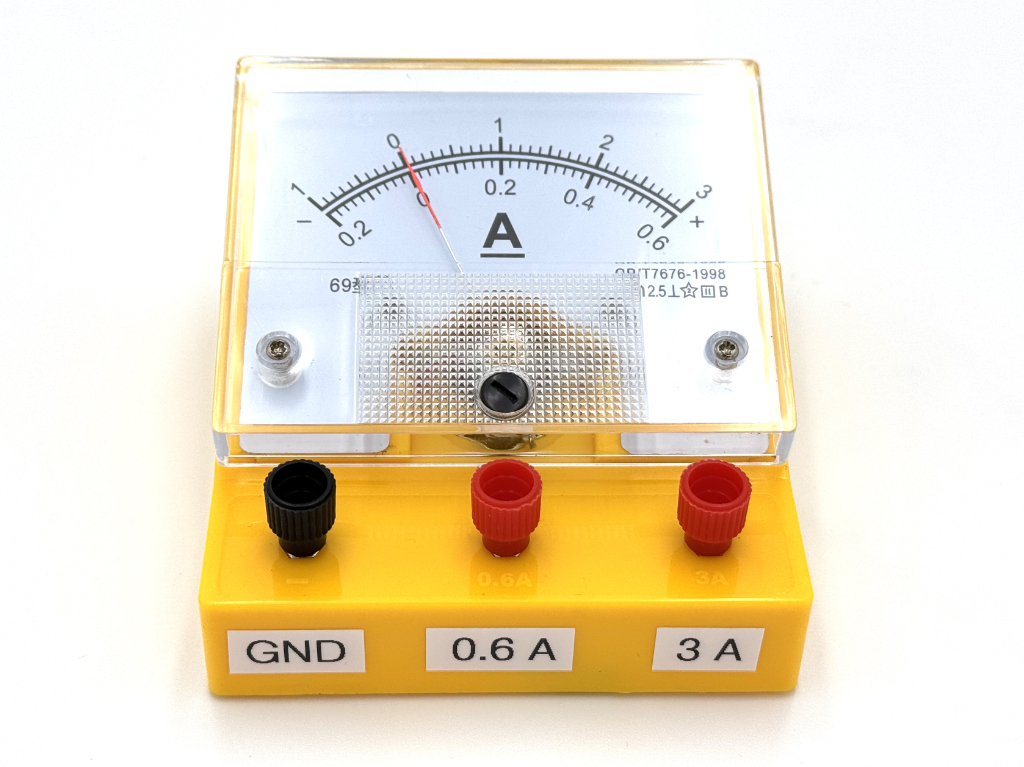
\includegraphics[width=6cm]{_images/ampere_meter}
    \caption{Stromstärkemessgerät, auch Amperemeter genannt.}
    \label{fig:amperemeter}
\end{figure}

Das Messgerät besteht aus einem Zeiger mit einer Skala, die die Stromstärke in Ampere darstellt.
Es hat drei Anschlüsse (GND), (0.6 A) und (3 A). Dies sind die beiden Messbereiche des Amperemeters.
Betrachtet man die Skala genau, sieht man, dass sie zweigeteilt ist. Die obere Skala zeigt
den Messbereich von -1 bis 3 Ampere, während die untere Skala den Bereich von -0.2 bis 0.6 Ampere abdeckt.


\newpage
\experiment{Stromstärkemessung}


Baue das Experiment aus siehe \fref{fig:current_measurement} auf.

\begin{figure}[h!]
    \centering
    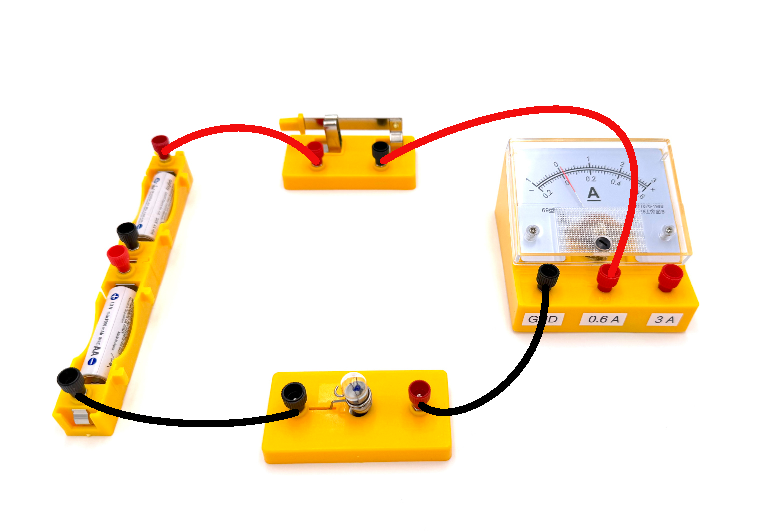
\includegraphics[width=9cm]{_images/ampere_setup.pdf}
    \caption{Stromstärkemessung}
    \label{fig:current_measurement}
\end{figure}

Schliesse den Schalter und notiere deine Beobachtungen. Beantworte die folgenden Fragen:

\begin{enumerate}
    \item Miss die Stromstärke mit dem Amperemeter (0.6 A).
    \item Miss die Stromstärke mit dem Amperemeter (3 A).
    \item Vertausche die beiden Kabel beim Amperemeter.
    \item Vervollständige den Schaltplan.
\end{enumerate}


% Raster für die Antworten
\begin{tikzpicture}
    \draw[step=4mm,gray,very thin] (0,0) grid (14.8,-8.4);

    \noanswer{
        \node  at (7,-6)
            {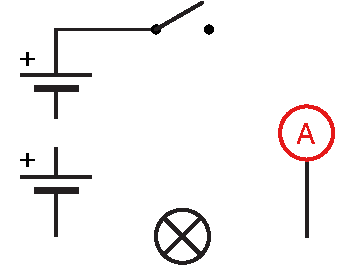
\includegraphics[width=6cm]{_images/ampere_setup_schaltplan.pdf}};
    }

    \answer{
        \node  at (7,-6)
            {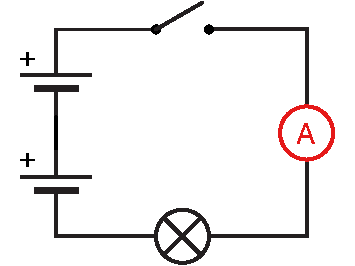
\includegraphics[width=6cm]{_images/ampere_setup_schaltplan_loesung.pdf}};
    }

    \answer{
        \draw (0.3,0.14) node[anchor=north west,align=left,text width=13cm] {%
      		\marker%

            \textbf{1.} Es fliessen ca. 0.26 A. \\
            \textbf{2.} Der Ausschlag der Nadel ist beim 3 A-Bereich kleiner Es fliesen etwas mehr als 0.2 A.\\
            \textbf{3.} Die Nadel schlägt in die negative Richtung aus.\\

        };
    }
\end{tikzpicture}


\newpage

\section{Kurzschluss bei der Stromstärkemessung}

Bei der Strommessung besteht die Gefahr, dass man das Amperemeter falsch anschliesst.
Es kann dann zu einem Kurzschluss kommen, welches in der Regel die Sicherung des
Amperemeters durchbrennen lässt, siehe \ref{fig:amperemeter_short_circuit}.

\begin{figure}[h!]
    \centering
    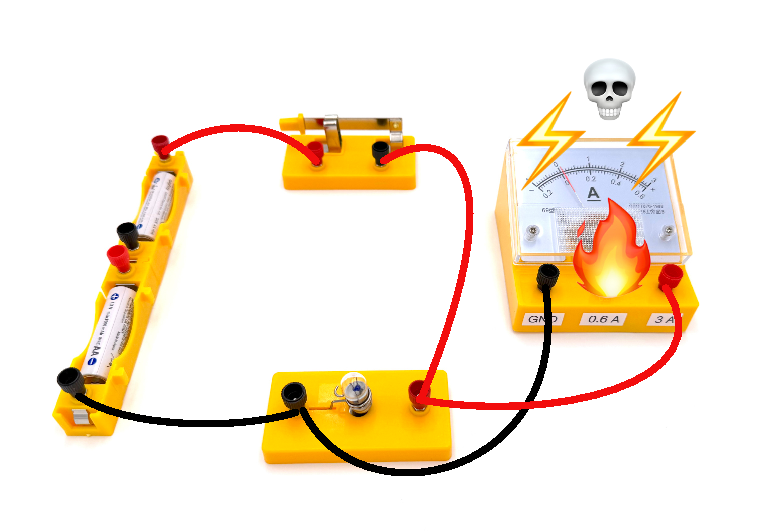
\includegraphics[width=8cm]{_images/ampere_kurzschluss}
    \caption{Kurzschluss mit dem Amperemeter}
    \label{fig:amperemeter_short_circuit}
\end{figure}

\begin{redbox}
Das Amperemeter darf nie parallel zum Verbraucher oder zur Batterie angeschlossen werden.
Es muss immer seriell, d.h. vor oder nach einem Verbraucher eingefügt werden.
\end{redbox}

Das Amperemeter hat die Aufgabe, den Stromfluss zu messen. Dafür muss es den elektrischen Strom
möglichst gut leiten. Man kann sich das Amperemeter wie ein Stück einer Leitung vorstellen.
Schaltet man das Amperemeter parallel zur Batterie, fliesst ein sehr grosser Strom
durch das Amperemeter und es entsteht ein Kurzschluss.


\exercise{Korrekte Stromstärkemessung}

Gib bei den folgenden Schaltplänen an, wo das Amperemeter richtig und wo falsch angeschlossen ist.

% Raster für die Antworten
\begin{tikzpicture}
    \draw[step=4mm,gray,very thin] (0,0) grid (14.8,-6);

    \node at (1,-0.6) {a)};
    \node  at (3.5,-3)
        {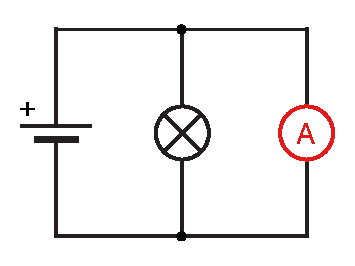
\includegraphics[width=6cm]{_images/ampere_kurzschluss_1.pdf}};

    \node at (8,-0.6) {b)};
    \node  at (10.5,-3)
        {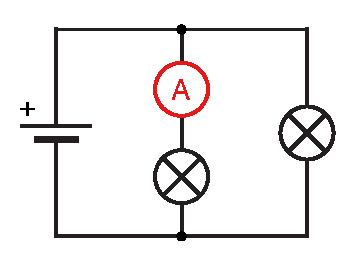
\includegraphics[width=6cm]{_images/ampere_kurzschluss_2.pdf}};

    \answer{
        \draw (1.4,-0.2) node[anchor=north west,align=left,text width=13cm] {%
      		\marker%
            falsch !! Achtung!
        };
        \draw (1.4,-5) node[anchor=north west,align=left,text width=13cm] {%
      		\marker%
        parallel zur Batterie!!!
        };


        \draw (8.4,-0.2) node[anchor=north west,align=left,text width=13cm] {%
      		\marker%
            korrekt
        };
        \draw (8.4,-5) node[anchor=north west,align=left,text width=13cm] {%
      		\marker%
            In Serie zum Verbraucher.
        };
    }
\end{tikzpicture}


\newpage
\experiment{Stromstärke in der Serienschaltung}

In diesem Experiment soll untersucht werden, wie gross die Stromstärke in einer Serienschaltung ist.
Das Amperemeter wird dazu nacheinander an verschiedenen Stellen im Stromkreis platziert.

\begin{figure}[h!]
\centering
    \begin{subfigure}[b]{0.305\textwidth}
    \centering
    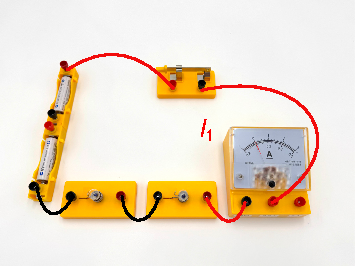
\includegraphics[width=4.6cm]{_images/ampere_serie_1.pdf}
    \end{subfigure}
\quad
    \begin{subfigure}[b]{0.305\textwidth}
    \centering
    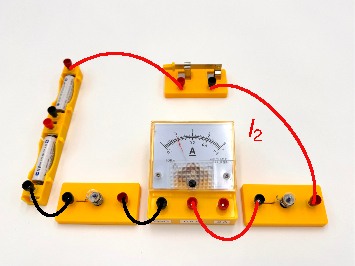
\includegraphics[width=4.6cm]{_images/ampere_serie_2.pdf}
    \end{subfigure}
\quad
    \begin{subfigure}[b]{0.305\textwidth}
    \centering
    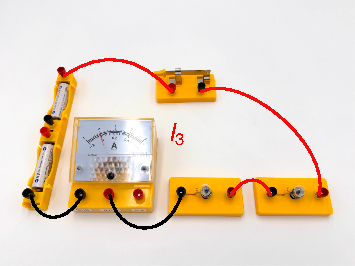
\includegraphics[width=4.6cm]{_images/ampere_serie_3.pdf}
    \end{subfigure}
\end{figure}


% Raster für die Antworten
\begin{tikzpicture}
    \draw[step=4mm,gray,very thin] (0,0) grid (14.8,-16);

    \node  at (3.5,-3.5)
        {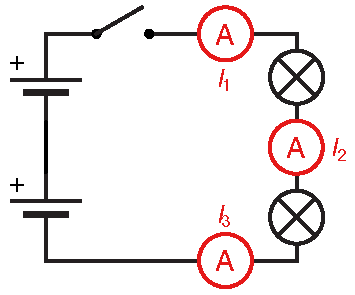
\includegraphics[width=6cm]{_images/ampere_serie}};

        \draw (8,-1.85) node[anchor=north west,align=left,text width=13cm] {%
      		\marker%

            I$_{\text{1}}$ = \answer{0.8 A}  \\
            I$_{\text{2}}$ = \answer{0.8 A} \\
            I$_{\text{3}}$ = \answer{0.8 A}  \\

        };

        \draw (1,-6.6) node[anchor=north west,align=left,text width=13cm] {%
      		\marker%

            Fazit\\
            \answer{Die Stromstärke in einer Serienschaltung ist überall\\
             gleich gross.}

        };
\end{tikzpicture}


\newpage
\experiment{Stromstärke in der Parallelschaltung}

In diesem Experiment werden die Stromstärken in einer Parallelschaltung untersucht.
Es wird die Gesamtstromstärke der beiden Lampen gemessen. Anschliessend wird das
Amperemeter nacheinander vor den einzelnen Lampen eingebaut.

\begin{figure}[h!]
\centering
    \begin{subfigure}[b]{0.305\textwidth}
    \centering
    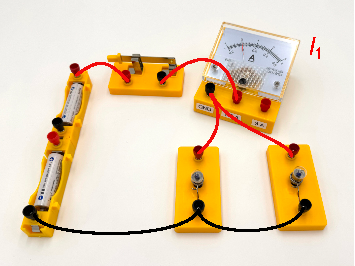
\includegraphics[width=4.6cm]{_images/ampere_parallel_1.pdf}
    \end{subfigure}
\quad
    \begin{subfigure}[b]{0.305\textwidth}
    \centering
    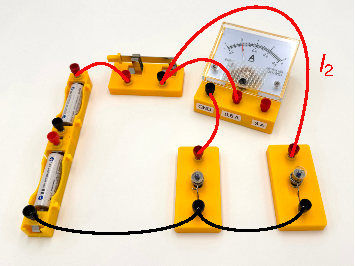
\includegraphics[width=4.6cm]{_images/ampere_parallel_2.pdf}
    \end{subfigure}
\quad
    \begin{subfigure}[b]{0.305\textwidth}
    \centering
    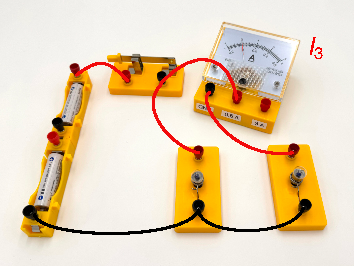
\includegraphics[width=4.6cm]{_images/ampere_parallel_3.pdf}
    \end{subfigure}
\end{figure}


% Raster für die Antworten
\begin{tikzpicture}
    \draw[step=4mm,gray,very thin] (0,0) grid (14.8,-14);

    \node  at (3.5,-3.5)
        {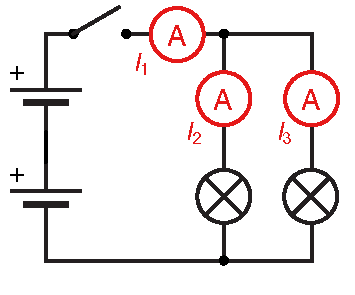
\includegraphics[width=6cm]{_images/ampere_parallel}};

        \draw (8,-1.85) node[anchor=north west,align=left,text width=13cm] {%
      		\marker%

            I$_{\text{1}}$ = \answer{0.44 A}  \\
            I$_{\text{2}}$ = \answer{0.22 A} \\
            I$_{\text{3}}$ = \answer{0.22 A}  \\

        };

        \draw (1,-6.6) node[anchor=north west,align=left,text width=13cm] {%
      		\marker%

            Fazit\\
            \answer{Die Stromstärke vor dem Knoten ist gleich der Summe der Stromstärken
            nach dem Knoten.}

        };
\end{tikzpicture}


\section{Spannungsmessung}

Die elektrische Spannung $U$ ist definiert als das Verhältnis zwischen der Energie $E$ und der Ladung $Q$.
Sie gibt an, wie viel elektrische Energie umgewandelt wird, wenn eine Ladungseinheit geflossen ist.
Die Einheit der Spannung ist das Volt ($\unit{\volt}$).

\begin{greenbox}
\textbf{Spannung $U$}
$$
    U = \frac{E}{Q} \quad,\quad \left[ U \, \right] = \frac{\unit{\joule}}{\unit{\coulomb}} = \unit{\volt} \quad \text{(Volt)}
$$
\end{greenbox}

\begin{figure}[h!]
    \centering
    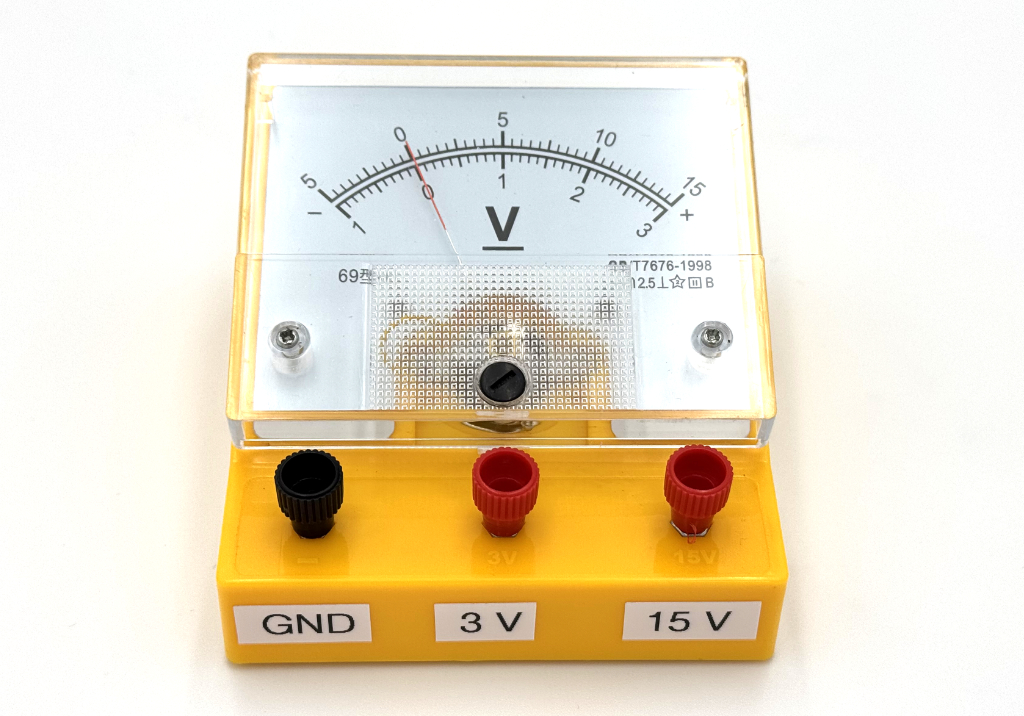
\includegraphics[width=8cm]{_images/volt_meter}
    \caption{Spannungsmessgerät, auch Voltmeter genannt.}
    \label{fig:voltmeter}
\end{figure}

Das Voltmeter ist ein Instrument, das die Spannung zwischen zwei Punkten in einem
elektrischen Kreis messen kann.

\begin{greenbox}
Spannungsmessgeräte werden immer parallel zum Verbraucher angeschlossen.
\end{greenbox}




\exercise{Korrekte Spannungsmessung}

Gib bei den folgenden Schaltplänen an, wo das Voltmeter richtig oder falsch angeschlossen ist.

% Raster für die Antworten
\begin{tikzpicture}
    \draw[step=4mm,gray,very thin] (0,0) grid (14.8,-6.41);

    \node at (1,-0.6) {a)};
    \node  at (3.5,-3)
        {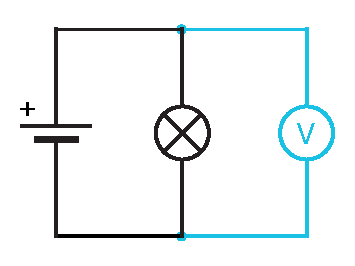
\includegraphics[width=6cm]{_images/volt_messung_1.pdf}};

    \node at (8,-0.6) {b)};
    \node  at (10.5,-3)
        {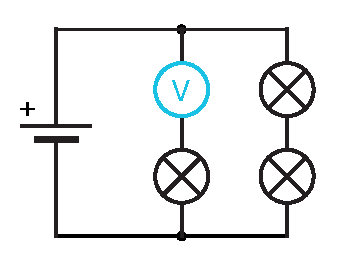
\includegraphics[width=6cm]{_images/volt_messung_2.pdf}};

    \answer{
        \draw (1.4,-0.2) node[anchor=north west,align=left,text width=13cm] {%
      		\marker%
        korrekt
        };
        \draw (1.4,-5) node[anchor=north west,align=left,text width=13cm] {%
      		\marker%
        Parallel zum Verbraucher\\
        ist korrekt.
        };


        \draw (8.4,-0.2) node[anchor=north west,align=left,text width=13cm] {%
      		\marker%
        falsch
        };
        \draw (8.4,-5) node[anchor=north west,align=left,text width=13cm] {%
      		\marker%
            In Serie zum Verbraucher\\
            ist falsch.
        };
    }
\end{tikzpicture}





\newpage
\experiment{Spannungsmessung}


Baue das Experiment aus siehe \fref{fig:voltage_measurement} auf.

\begin{figure}[h!]
    \centering
    \includegraphics[width=9cm]{_images/volt_setup.pdf}
    \caption{Spannungsmessung}
    \label{fig:voltage_measurement}
\end{figure}

Schliesse den Schalter und notiere deine Beobachtungen. Beantworte die folgenden Fragen:

\begin{enumerate}
    \item Miss die Spannung mit dem Voltmeter (3 V).
    \item Miss die Spannung mit dem Voltmeter (15 A).
    \item Vertausche die beiden Kabel beim Voltmeter.
    \item Vervollständige den Schaltplan.
\end{enumerate}


% Raster für die Antworten
\begin{tikzpicture}
    \draw[step=4mm,gray,very thin] (0,0) grid (14.8,-8.4);

    \noanswer{
        \node  at (7,-6)
            {\includegraphics[width=6cm]{_images/volt_setup_schaltplan.pdf}};
    }

    \answer{
        \node  at (7,-6)
            {\includegraphics[width=6cm]{_images/volt_setup_schaltplan_loesung.pdf}};
    }

    \answer{
        \draw (0.3,0.14) node[anchor=north west,align=left,text width=13cm] {%
      		\marker%

            \textbf{1.} Die Spannung beträgt ca. 2.4 V. \\
            \textbf{2.} Der Ausschlag der Nadel ist beim 15 V-Bereich kleiner. Die Spannung beträgt aber immer noch ca. 2.4 V.\\
            \textbf{3.} Die Nadel schlägt in die negative Richtung aus.\\

        };
    }
\end{tikzpicture}





\newpage
\experiment{Spannung in der Serienschaltung}

In diesem Experiment soll untersucht werden, wie gross die Spannungen in einer Serienschaltung sind.
Das Voltmeter wird dazu nacheinander an verschiedenen Stellen im Stromkreis platziert.

\begin{figure}[h!]
\centering
    \begin{subfigure}[b]{0.305\textwidth}
    \centering
    \includegraphics[width=4.6cm]{_images/volt_serie_1.pdf}
    \end{subfigure}
\quad
    \begin{subfigure}[b]{0.305\textwidth}
    \centering
    \includegraphics[width=4.6cm]{_images/volt_serie_2.pdf}
    \end{subfigure}
\quad
    \begin{subfigure}[b]{0.305\textwidth}
    \centering
    \includegraphics[width=4.6cm]{_images/volt_serie_3.pdf}
    \end{subfigure}
\end{figure}


% Raster für die Antworten
\begin{tikzpicture}
    \draw[step=4mm,gray,very thin] (0,0) grid (14.8,-16);

    \node  at (3.5,-3.5)
        {\includegraphics[width=7cm]{_images/volt_serie}};

        \draw (8,-1.85) node[anchor=north west,align=left,text width=13cm] {%
      		\marker%

            U$_{\text{1}}$ = \answer{2.4 V}  \\
            U$_{\text{2}}$ = \answer{1.2 V} \\
            U$_{\text{3}}$ = \answer{1.2 V}  \\

        };

        \draw (1,-6.6) node[anchor=north west,align=left,text width=12cm] {%
      		\marker%

            Fazit\\
            \answer{Die Spannung U$_{\text{1}}$ über beiden Lampen zusammen ist die Summe aus den
            Spannungen U$_{\text{2}}$ und U$_{\text{3}}$ über den einzelnen Lampen.}

        };
\end{tikzpicture}



\newpage
\experiment{Spannungsmessung in der Parallelschaltung}

In diesem Experiment werden die Spannungen in einer Parallelschaltung untersucht.
Dazu werden die Spannungen über die einzelnen Lampen gemessen.

\begin{figure}[h!]
\centering
    \begin{subfigure}[b]{0.305\textwidth}
    \centering
    \includegraphics[width=4.6cm]{_images/volt_parallel_1.pdf}
    \end{subfigure}
\quad
    \begin{subfigure}[b]{0.305\textwidth}
    \centering
    \includegraphics[width=4.6cm]{_images/volt_parallel_2.pdf}
    \end{subfigure}
\quad
        \begin{subfigure}[b]{0.305\textwidth}
        \centering
        \includegraphics[width=4.6cm]{_images/volt_parallel_3.pdf}
        \end{subfigure}
\end{figure}


% Raster für die Antworten
\begin{tikzpicture}
    \draw[step=4mm,gray,very thin] (0,0) grid (14.8,-14);

    \node  at (4,-3.5)
        {\includegraphics[width=8cm]{_images/volt_parallel}};

        \draw (9,-1.85) node[anchor=north west,align=left,text width=13cm] {%
      		\marker%

            U$_{\text{1}}$ = \answer{2.4 V}  \\
            U$_{\text{2}}$ = \answer{2.4 V} \\
            U$_{\text{3}}$ = \answer{2.4 V} \\

        };

        \draw (1,-6.6) node[anchor=north west,align=left,text width=12cm] {%
      		\marker%

            Fazit\\
            \answer{Bei der Parallelschaltung sind die Spannungen U$_{\text{2}}$ und U$_{\text{3}}$ über den beiden Lampen gleich gross, wie die Spannung U$_{\text{1}}$ der Batterie.}

        };
\end{tikzpicture}



\newpage
\chapter{Ohmsches Gesetz}


Bis jetzt haben wir uns mit der Stromstärke- und Spannungsmessung beschäftigt.
Man kann sich nun die Frage stellen, ob die Spannung und die Stromstärke
unabhängig voneinander sind oder nicht.

Denkt man an das Modell des Wasserkreislaufs, siehe \fref{fig:watermodel},
so wird klar, dass die Höhe des Wassers im Tank einen Einfluss auf die
Flussgeschwindigkeit des Wassers in den Röhren hat.
Es könnte also plausibel sein, dass die Spannung und die Stromstärke nicht
unabhängig voneinander sind.

\section{Der Schiebewiderstand}

Ein Schiebewiderstand ist ein elektrisches Bauteil, mit welchem man die Stromstärke
regulieren kann, siehe \fref{fig:potentiometer}. Er besteht aus einer gewickelten Spule
aus einem speziellen Widerstandsdraht und einem Schieber, der mit dieser Spule Kontakt hat.

\begin{figure}[h!]
    \centering
    \includegraphics[width=11cm]{_images/schiebewiderstand.pdf}
    \caption{Schiebewiderstand}
    \label{fig:potentiometer}
\end{figure}

Die Anschlüsse A und B sind miteinander und mit dem Schieber verbunden.
Die Anschlüsse der Spule sind bei C und D. Der Kontaktpunkt zwischen Schieber und Spule ist bei M.



\newpage
\experiment{Stromregulierung mit dem Schiebewiderstand}

Baue das Experiment aus siehe \fref{fig:potentiometer_series} auf.

\begin{figure}[h!]
    \centering
    \includegraphics[width=9cm]{_images/ohm_schiebewiderstand.pdf}
    \caption{Regulierung der Stromstärke mit dem Schiebewiderstand}
    \label{fig:potentiometer_series}
\end{figure}

Schliesse den Schalter und notiere deine Beobachtungen. Beantworte die folgenden Fragen:

\begin{enumerate}
    \item Miss die Stromstärke, wenn der Schieber ganz links ist.
    \item Miss die Stromstärke, wenn der Schieber in der Mitte ist.
    \item Miss die Stromstärke, wenn der Schieber ganz rechts ist.
    \item Vervollständige den Schaltplan.
\end{enumerate}


% Raster für die Antworten
\begin{tikzpicture}
    \draw[step=4mm,gray,very thin] (0,0) grid (14.8,-8.4);

    \noanswer{
        \node  at (7,-6)
            {\includegraphics[width=6cm]{_images/ohm_schiebewiderstand_schaltplan.pdf}};
    }

    \answer{
        \node  at (7,-6)
            {\includegraphics[width=6cm]{_images/ohm_schiebewiderstand_schaltplan_loesung.pdf}};
    }

    \answer{
        \draw (0.3,0.14) node[anchor=north west,align=left,text width=13cm] {%
      		\marker%

            \textbf{1.} Es fliessen ca. 0.26 A. \\
            \textbf{2.} Der Ausschlag der Nadel ist beim 3 A-Bereich kleiner Es fliesen etwas mehr als 0.2 A.\\
            \textbf{3.} Die Nadel schlägt in die negative Richtung aus.\\

        };
    }
\end{tikzpicture}






\newpage
\experiment{Zusammenhang zwischen Spannung und Stromstärke}

Baue das Experiment aus siehe \fref{fig:ohm_law} auf. Es gibt vier verschiedene
Widerstände auf dem Brettchen. Verbinde zuerst den zweitobersten
Widerstand ($\qty{10}{\ohm}$), danach den untersten ($\qty{20}{\ohm}$).

\begin{figure}[h!]
    \centering
    \includegraphics[width=9cm]{_images/ohm_gesetz.pdf}
    \caption{Strom- und Spannungsmessung über einem Widerstand.}
    \label{fig:ohm_law}
\end{figure}

Schliesse den Schalter und verändere den Schiebewiderstand. Miss vier verschiedene
Kombinationen von Spannung und Stromstärke. Zeichne anschliessend die Messwerte
in das Diagramm.

% Raster für die Antworten
\begin{tikzpicture}
    \draw[step=4mm,gray,very thin] (0,0) grid (14.8,-11.6);


    \begin{scope}[shift={(1.2,0)}]
    \draw (2.2,-0.6) node[anchor=north east,align=right,text width=3cm] {%
  		\markertable%
        U in V
        \ \\
        10 Ω , I in A
        \ \\
        20 Ω , I in A
        \ \\
    };

    \draw[very thick] (0.8,-1.6) -- (10.8,-1.6);

    \draw[very thick] (2.8,-0.4) -- ++(0,-3.6);

    \draw (3.6,-0.6) node[anchor=north,align=center,text width=2cm] {%
  		\markertable%
        0
        \ \\
        \answer{0}
        \ \\
        \answer{0}
        \ \\
    };


    \draw[very thick] (4.4,-0.4) -- ++(0,-3.6);

    \draw (5.2,-0.6) node[anchor=north,align=center,text width=2cm] {%
  		\markertable%
        0.5
        \ \\
        \answer{0.05}
        \ \\
        \answer{0}
        \ \\
    };

    \draw[very thick] (6,-0.4) -- ++(0,-3.6);

    \draw (6.8,-0.6) node[anchor=north,align=center,text width=2cm] {%
  		\markertable%
        1
        \ \\
        \answer{0.1}
        \ \\
        \answer{0}
        \ \\
    };

    \draw[very thick] (7.6,-0.4) -- ++(0,-3.6);

    \draw (8.4,-0.6) node[anchor=north,align=center,text width=2cm] {%
  		\markertable%
        1.5
        \ \\
        \answer{0.15}
        \ \\
        \answer{0}
        \ \\
    };

    \draw[very thick] (9.2,-0.4) -- ++(0,-3.6);

    \draw (10,-0.6) node[anchor=north,align=center,text width=2cm] {%
  		\markertable%
        \answer{2.2}
        \ \\
        \answer{0.22}
        \ \\
        \answer{0}
        \ \\
    };
    \end{scope}



    \begin{scope}[shift={(4,-10)}]
        \draw[color=white,fill=white] (-1,-1) rectangle (7,5);
        \begin{axis}[
                axis background/.style={fill=white},
                axis lines=left,
                xlabel=$I$ in A,
                ylabel=$U$ in V,
                xtick={0,0.1,0.2,0.3,0.4},
                ytick={0,1,2,3},
                minor tick num=1,
                grid=both,
                xmin=0.0, xmax=0.3,
                ymin=0, ymax=3,
                line width=1pt,
                height=6cm,
                width=8cm,
                domain=0:0.3,
                legend pos=south east
            ]
            \answer{
                \addplot[
                    mark=*, mark size=1.5,color=blue,
                ] coordinates
                {
                    (0,0)
                    (0.05, 0.5)
                    (0.1,1)
                    (0.15,1.5)
                    (0.22,2.2)
                };
                \addplot[
                    mark=*, mark size=1.5,color=red,
                ] coordinates
                {
                    (0,0)
                    (0.033, 0.5)
                    (0.067,1)
                    (0.1,1.5)
                    (0.15,2.2)
                };
                \legend{10 Ω,20 Ω}
            }
        \end{axis}
    \end{scope}

\end{tikzpicture}






\newpage
\section{Der elektrische Widerstand}

Der elektrische Widerstand $R$ ist definiert als das Verhältnis zwischen
der Spannung $U$ und der Stromstärke $I$. Die Einheit des Widerstands ist
das Ohm ($\unit{\ohm}$).

\begin{greenbox}
\textbf{Elektrischer Widerstand $R$}
$$
    R = \frac{U}{I} \quad,\quad \left[ R \, \right] = \frac{\unit{\volt}}{\unit{\ampere}} = \unit{\ohm} \quad \text{(Ohm)}
$$
\end{greenbox}

Der elektrische Widerstand ist ein Mass für die elektrische Widerstandsfähigkeit
eines Materials oder einer elektrischen Komponente. Ohmsche Widerstände führen
zur Umwandlung von elektrischer Energie in Wärme.

Wenn man die Spannung $U$ über einem Widerstand $R$ erhöht, erhöht sich auch die Stromstärke $I$.
Normalerweise wird dann auch die Leistung $P$ grösser, was zu einer Erwärmung des Widerstands führt.
Diese wiederum verändert den elektrischen Widerstand.

\begin{greenbox}
\textbf{Das Ohmsche Gesetz}\\

Die Spannung $U$ über einem ohmschen Widerstand $R$ ist proportional zur Stromstärke $I$.
Mit anderen Worten, der elektrische Widerstand bleibt konstant.
$$
    R = \frac{U}{I} = \text{const.}
$$
\end{greenbox}

In der Regel gilt das Ohmsche Gesetz nur näherungsweise, da sich alle Materialien bei
höherem Stromdurchfluss erwärmen.


\experiment{Messung des unbekannten Widerstands}

Auf dem Widerstandsbrettchen hat es einen Widerstand, der nicht
angeschrieben ist. Bestimme durch eine Messung dessen Wert. Vervollständige
anschliessend den Schaltplan.

% Raster für die Antworten
\begin{tikzpicture}
    \draw[step=4mm,gray,very thin] (0,0) grid (14.8,-8);

    \answer{
        \draw (0.8,-0.2) node[anchor=north west,align=left,text width=12cm] {%
      		\marker%

            Gemessen: U=2 V, I=130 mA\\
            \ \\
            R = U/I = 2 V / 0.13 A = 15 Ω
        };
    }

    \noanswer{
        \node  at (7,-5.4)
            {\includegraphics[width=6cm]{_images/ohm_widerstand_schaltplan.pdf}};
    }

    \answer{
        \node  at (7,-5.4)
            {\includegraphics[width=6cm]{_images/ohm_widerstand_schaltplan_loesung.pdf}};
    }
\end{tikzpicture}









\newpage
\experiment{Kennlinie einer Glühbirne}

Baue das Experiment aus siehe \fref{fig:ohm_lampe} auf. Stelle mit dem
Schiebewiderstand verschiedene Spannungen ein und miss jeweils die Stromstärke.


\begin{figure}[h!]
    \centering
    \includegraphics[width=9cm]{_images/ohm_lampe.pdf}
    \caption{Strom- und Spannungsmessung über einem Glühbirne.}
    \label{fig:ohm_lampe}
\end{figure}

Erstelle aus den Messdaten die Widerstandskennlinie der Glühbirne.
Wie unterscheiden sie sich von der Kennlinie der Widerstände?


% Raster für die Antworten
\begin{tikzpicture}
    \draw[step=4mm,gray,very thin] (0,0) grid (14.8,-11.6);


    \begin{scope}[shift={(1.2,0)}]
    \draw (2.2,-0.6) node[anchor=north east,align=right,text width=3cm] {%
  		\markertable%
        U in V
        \ \\
        I in A
        \ \\
    };

    \draw[very thick] (0.8,-1.6) -- ++(10,0);

    \draw[very thick] (2.8,-0.4) -- ++(0,-2.4);

    \draw (3.6,-0.6) node[anchor=north,align=center,text width=2cm] {%
  		\markertable%
        0
        \ \\
        \answer{0}
        \ \\
    };


    \draw[very thick] (4.4,-0.4) -- ++(0,-2.4);

    \draw (5.2,-0.6) node[anchor=north,align=center,text width=2cm] {%
  		\markertable%
        0.5
        \ \\
        \answer{0.13}
        \ \\
    };

    \draw[very thick] (6,-0.4) -- ++(0,-2.4);

    \draw (6.8,-0.6) node[anchor=north,align=center,text width=2cm] {%
  		\markertable%
        1
        \ \\
        \answer{0.16}
        \ \\
    };

    \draw[very thick] (7.6,-0.4) -- ++(0,-2.4);

    \draw (8.4,-0.6) node[anchor=north,align=center,text width=2cm] {%
  		\markertable%
        1.5
        \ \\
        \answer{0.2}
        \ \\
    };

    \draw[very thick] (9.2,-0.4) -- ++(0,-2.4);

    \draw (10,-0.6) node[anchor=north,align=center,text width=2cm] {%
  		\markertable%
        \answer{2.2}
        \ \\
        \answer{0.24}
        \ \\
    };
    \end{scope}

    \noanswer{
        \draw (0.3,-10.2) node[anchor=north west,align=left,text width=13cm] {%
      		\marker%
            Fazit:
        };
    }

    \answer{
        \draw (0.3,-9.8) node[anchor=north west,align=left,text width=13cm] {%
      		\marker%
            Fazit: Der elektrische Widerstand einer Glühbirne ist nicht\\
            konstant. Je heller sie brennt, desto höher ist der Widerstand.\\
        };
    }



    \begin{scope}[shift={(4,-8.4)}]
        \draw[color=white,fill=white] (-1,-1) rectangle (7,5);
        \begin{axis}[
                axis background/.style={fill=white},
                axis lines=left,
                xlabel=$I$ in A,
                ylabel=$U$ in V,
                xtick={0,0.1,0.2,0.3,0.4},
                ytick={0,1,2,3},
                minor tick num=1,
                grid=both,
                xmin=0.0, xmax=0.3,
                ymin=0, ymax=3,
                line width=1pt,
                height=6cm,
                width=8cm,
                domain=0:0.3,
            ]
            \answer{
                \addplot[
                    only marks,
                    mark=*,
                    mark size=1.5,
                    color=blue,
                ] coordinates
                {
                    (0,0)
                    (0.13, 0.5)
                    (0.16,1)
                    (0.2,1.5)
                    (0.24,2.2)
                };

                \addplot[
                    color=red,
                    domain=0:0.3,
                ] {43.736*x^2 - 1.2614*x};
            }
        \end{axis}
    \end{scope}

\end{tikzpicture}








\newpage
\experiment{Serieschaltung von Widerständen}

Baue das Experiment aus siehe \fref{fig:ohm_resistors_series} auf.

\begin{figure}[h!]
    \centering
    \includegraphics[width=6cm]{_images/ohm_widerstand_serie.pdf}
    \caption{Serieschaltung von Widerständen.}
    \label{fig:ohm_resistors_series}
\end{figure}

\begin{enumerate}
    \item Miss den Gesamtwiderstand der beiden Widerständen.
    \item Leite eine Formel für den Gesamtwiderstand her.
    \item Überprüfe deine Formel mit den anderen Widerständen.
\end{enumerate}

% Raster für die Antworten
\begin{tikzpicture}
    \draw[step=4mm,gray,very thin] (0,0) grid (14.8,-11.6);

    \answer{
        \draw (0.3,-0.4) node[anchor=north west,align=left,text width=13cm] {%
      		\marker%
            Die Messungen zeigen, dass der Gesamtwiderstand der beiden
            seriellen Widerstände gleich der Summe der beiden Widerstände ist.

            Die Formel lautet:
            $$
            R_{ges} = R_1 + R_2
            $$
        };
    }

\end{tikzpicture}




\newpage
\experiment{Parallelschaltung von Widerständen}

Baue das Experiment aus siehe \fref{fig:ohm_resistors_parallel} auf.

\begin{figure}[h!]
    \centering
    \includegraphics[width=6cm]{_images/ohm_widerstand_parallel.pdf}
    \caption{Parallelschaltung von Widerständen.}
    \label{fig:ohm_resistors_parallel}
\end{figure}

\begin{enumerate}
    \item Miss den Gesamtwiderstand der beiden Widerständen.
    \item Leite eine Formel für den Gesamtwiderstand her.
    \item Überprüfe deine Formel mit den anderen Widerständen.
\end{enumerate}

% Raster für die Antworten
\begin{tikzpicture}
    \draw[step=4mm,gray,very thin] (0,0) grid (14.4,-11.6);

    \answer{
        \draw (0.3,-0.4) node[anchor=north west,align=left,text width=13cm] {%
      		\marker%
            Die Messungen zeigen, dass der Gesamtwiderstand der beiden
            parallelen Widerstände kleiner ist als der kleinere der beiden Widerstände.

            Man kann die folgenden Formeln herleiten:
            $$
            \frac{1}{R_{ges}} = \frac{1}{R_1} + \frac{1}{R_2}
            $$
            oder umgeformt:
            $$
            R_{ges} = \frac{R_1 * R_2}{R_1 + R_2}
            $$
        };
    }



\end{tikzpicture}

\newpage
\section{Die elektrische Leistung}


Die elektrische Leistung $P$ ist definiert als das Produkt der Spannung $U$ und der Stromstärke $I$. Die Einheit der Leistung ist
das Watt ($\unit{\watt}$).


\begin{greenbox}
\textbf{Elektrische Leistung $P$}
$$
    P = U * I \quad,\quad \left[ P \, \right] = \unit{\volt} * \unit{\ampere} = \unit{\watt} \quad \text{(Watt)}
$$
\end{greenbox}



\exercise{Formel herleiten}

Die Leistung $P$ ist das Verhältnis der Energie $E$ zu der Zeit $t$.
Zeige, dass das Produkt aus Spannung und Stromstärke gleich der Leistung ist.
Überprüfe anschliessend auch die Einheiten, d.h. zeige, dass Volt mal Ampere gleich Watt ist.

% Raster für die Antworten
\begin{tikzpicture}
    \draw[step=4mm,gray,very thin] (0,0) grid (14.8,-4);

    \answer{
        \draw (0.3,-0.4) node[anchor=north west,align=left,text width=13cm] {%
      		\marker%
            $$
                U * I = \frac{E}{Q} * \frac{Q}{t} = \frac{E}{t} = P
            $$

            $$
                \unit{\volt} * \unit{\ampere} = \frac{\unit{\joule}}{\unit{\coulomb}} * \frac{\unit{\coulomb}}{\unit{\second}} = \frac{\unit{\joule}}{\unit{\second}} = \unit{\watt}
            $$
        };
    }

\end{tikzpicture}



\exercise{P-I-Diagramm einer Glühbirne}

Erstelle ein Diagramm der Leistung $P$ einer Glühbirne als Funktion der Stromstärke $I$.
Verwende dazu die Formel $P = U * I$ und die Werte für die Spannung $U$ und die
Stromstärke $I$ der Glühbirne.

% Raster für die Antworten
\begin{tikzpicture}
    \draw[step=4mm,gray,very thin] (0,0) grid (14.8,-8);

    \begin{scope}[shift={(4,-6)}]
        \draw[color=white,fill=white] (-1.5,-1) rectangle (7.5,5);
        \begin{axis}[
                axis background/.style={fill=white},
                axis lines=left,
                xlabel=$I$ in A,
                ylabel=$P$ in W,
                xtick={0,0.1,0.2,0.3,0.4},
                ytick={0,0.2,0.4,0.6},
                minor tick num=1,
                grid=both,
                xmin=0.0, xmax=0.3,
                ymin=0, ymax=0.6,
                line width=1pt,
                height=6cm,
                width=8cm,
                domain=0:0.3,
            ]
            \answer{
                \addplot[
                    only marks,
                    mark=*,
                    mark size=1.5,
                    color=blue,
                ] coordinates
                {
                    (0,0)
                    (0.13, 0.065)
                    (0.16,0.16)
                    (0.2,0.3)
                    (0.24,0.528)
                };

                \answer{
                    \addplot[
                        color=red,
                        domain=0:0.3,
                    ] {8*x^2};
                }
            }
        \end{axis}
    \end{scope}

\end{tikzpicture}

\newpage
\chapter{Schlusswort}

In diesem Praxisheft hast du die Grundlagen der Elektrizitätslehre kennengelernt.
Du hast erfahren, wie elektrische Ströme fliessen, wie Spannung und Stromstärke
zusammenhängen und wie sich Widerstände und elektrische Leistung im Stromkreis verhalten.
Mit vielen Experimenten konntest du selbst entdecken, wie Elektrizität in der Praxis
funktioniert – vom einfachen Stromkreis bis hin zu komplexeren Schaltungen.

Die elektrische Energie begegnet uns täglich – in Lampen, Handys, Computern
oder in der Bahn. Umso wichtiger ist es, zu verstehen, wie sie entsteht,
wie man sie nutzt und worauf man achten muss, damit alles sicher bleibt.

Vielleicht hast du beim Experimentieren gemerkt, dass in der Physik nicht
nur Theorie, sondern auch viel Neugier, genaues Beobachten und selbstständiges
Denken gefragt ist. Genau das macht die Naturwissenschaften spannend – und manchmal
auch ein bisschen herausfordernd.

Dieses Heft ist ein Anfang. Wenn du Lust hast, kannst du dich noch weiter mit
Elektrizität beschäftigen – z. B. mit elektrischen Schaltungen in der Technik,
dem Aufbau von Stromnetzen oder den faszinierenden Möglichkeiten erneuerbarer Energien.

\chapter{Glossar}

\begin{description}
    \item[Stromstärke] Die elektrische Stromstärke $I$ gibt an, wie viel elektrische Ladung pro Zeit durch einen Leiter fliesst. Gemessen in Ampere ($\unit{\ampere}$).

    \item[Spannung] Die elektrische Spannung $U$ ist die Ursache für den Fluss von elektrischem Strom. Sie wird in Volt ($\unit{\volt}$) gemessen.

    \item[Widerstand] Der elektrische Widerstand $R$ beschreibt, wie stark ein Bauteil den Stromfluss hemmt. Gemessen in Ohm ($\unit{\ohm}$).

    \item[Leistung] Die elektrische Leistung $P$ ist das Produkt aus Spannung und Stromstärke. Sie wird in Watt ($\unit{\watt}$) gemessen.

    \item[seriell] Schaltung, bei der die Bauteile hintereinander in einem einzigen Stromkreis verbunden sind. Die Stromstärke ist überall gleich.

    \item[parallel] Schaltung, bei der die Bauteile nebeneinander in verschiedenen Stromkreisen verbunden sind. Die Spannung ist überall gleich.
\end{description}


\end{document}
